\documentclass{wrcecapstone}

% Known issues:
% Does not incorporate Dr Allison Webster Giddings comments from end of EW401

\usepackage[separate-uncertainty=true,multi-part-units=single]{siunitx}
\DeclareSIUnit{\year}{y}
\DeclareSIUnit{\inch}{in}
\DeclareSIUnit{\foot}{ft}
\DeclareSIUnit{\poundforce}{lbf}
\DeclareSIUnit{\pound}{lb}
\DeclareSIUnit{\frame}{frame}
\DeclareSIUnit{\mph}{mph}
\DeclareSIUnit{\mile}{mi}
\DeclareSIUnit{\nauticalmile}{nm}
\DeclareSIUnit{\fahrenheit}{F}
\usepackage{graphicx} % covered in WRCE capstone
\usepackage[noadjust]{cite}
\bibliographystyle{IEEEtran}
\usepackage[plain]{fancyref}
\usepackage{amsmath,amsfonts,amssymb}
\usepackage{booktabs}
\usepackage{listings}
\lstset{%
  basicstyle=\ttfamily,
  columns=fullflexible,
  showstringspaces=false}
\lstdefinestyle{mbedC}{
	language=C,
	basicstyle=\ttfamily,
	keywordstyle=\color{blue}\ttfamily,
	stringstyle=\color{magenta}\ttfamily,
	commentstyle=\color{green}\ttfamily,
	directivestyle=\color{red}\ttfamily,
 	morecomment=[l][\color{red}]{\#},
	columns=fullflexible,
	showstringspaces=false,
%	frame=single
}
\lstdefinestyle{usnaMatlab}{
	basicstyle=\ttfamily,
	keywordstyle=\color{blue}\ttfamily,
	stringstyle=\color{magenta}\ttfamily,
	commentstyle=\color{green}\ttfamily,
 	morecomment=[l][\color{red}]{\#},
	columns=fullflexible,
	showstringspaces=false,
	language=Matlab
%	%backgroundcolor=\color{lightgray},
%	frame=single
}
%\usepackage[dvipsnames,svgnames]{xcolor} % partially covered in WRCE capstone
%\usepackage{hyperref} % covered in WRCE capstone
%\hypersetup{%
%  colorlinks=true,
%  linkcolor=violet,
%  urlcolor=blue,
%  citecolor=blue}
%\usepackage{fullpage}
\usepackage{svg}
%\usepackage{svg-extract}
\usepackage[inputamerican,english,cleanlook]{isodate}

\newcommand{\Matlab}{Matlab}
\newcommand{\Dudleyanesiotica}{\emph{Dudleya nesiotica}}
\newcommand{\Dnesiotica}{\emph{D.~nesoitica}}
\newcommand{\Dudleya}{\emph{Dudleya}}
\newcommand{\Malvaassurgentiflora}{\emph{Malva assurgentiflora}}
\newcommand{\Massurgentiflora}{\emph{M.~assurgentiflora}}
\newcommand{\Malva}{\emph{Malva}}

\title{Biomechanics Secure Terrestrial {\nobreak Ecological} Vegetation Extractor (STEVE)}
\student{Midshipman~1/C~Reina~Carroll, Midshipman~1/C~Jacob~Kang, Midshipman~1/C~Ji~Lim, Midshipman ~1/C~Bryan~Phan, and Midshipman~2/C~Levi~Hofland}
\author{Reina~Carroll, Jacob~Kang, Ji~Lim, Bryan~Phan, and Levi~Hofland}
%\contactinfo{bryanphan168@gmail.com, jmkang1998@gmail.com, jlim225@gmail.com, reinscarroll@gmail.com, samsgaffer@gmail.com}
\advisor{Assistant Professor D.~Evangelista}
\departmentchair{Professor B.~Bishop}
\date{\today}

\begin{document}
\maketitlepage
\cleardoublepage
\tableofcontents
\listoffigures
\listoftables

% first page
\clearpage
\maketitle


\begin{abstract}
Environmental and ecological research are often constrained by the accessibility of desired areas to obtain samples. In botanical fields of study, there has been an increased use of unmanned aerial systems (UAS) for surveying and identifying plants growing in these inaccessible areas. However, there is minimal research in UAS plant collection. We will discuss the development of a UAS attached with an extraction device by considering the system’s operating time, payload capacity, reliability of extraction, and resistance to the forces of nature. Our design is focused on development in radio/control, software engineering, electrically powered mechanical systems, cutting methods for plants, 3D printing, and UAS flight operations. The location and geography of the operation environment motivates the designs of the project. We will present concept designs and initial prototyping for the operation mission: (1) to survey a specified area for expert botanist to identify desired plants; (2) to reach to the desired plant in the inaccessible location; and (3) to extract, secure, and recover a sample of the plant from the inaccessible location. We will also discuss the logistics and qualifications required for the team and plans for the operation to support the botanist mission. The UAS design we develop is tailored towards the need of botanists and their research, and we envision further develop in the capabilities of the UAS to support potential missions in industry or the military.
\end{abstract}
\footnotetext{Bryan Phan, Jacob Kang, and Ji Lim are with the Department of Weapons, Robotics, and Control Engineering at the United States Naval Academy. Reina Carroll and Levi Hofland are with the Department of Mechanical Engineering. Addresses for correspondence: \emph{bryanphan168@gmail.com}, \emph{jmkang1998@gmail.com}, \emph{jlim225@gmail.com}, \emph{reinscarroll@gmail.com}, \emph{samsgaffer@gmail.com}}

\section{Introduction}

\subsection{Customer interview}
Dr. Matt Guilliams, a plant systematist and curator of the Santa Barbara Botanical Garden's Clifton Smith Herbarium, studies the flora of California including floristics, biodiversity description, inferring evolutionary patterns, and genetic conservation of rare plants. He is currently researching the endemic species of flora on the Channel Islands. Endemic refers to species of flora or fauna that only exists in specific areas of the world. Dr. Matt Guilliams wants to identify and collect samples of understudied species of flora on the Channel Islands off the coast of Santa Barbara because he seeks to protect the endemic plants of these islands.

Our team interviewed Dr. Guilliams through a phone call on \printdate{9/11/2019} in order to discuss his vision for the project and gain insights on the environment we will be working in. This interview highlighted that the species of plant we are trying to collect is located on the cliffside of the Channel Island, reaching heights up to 50 feet tall. The two species of plants that Dr. Guilliams is interested in is the \Malvaassurgentiflora\ and the \Dudleyanesiotica\ plants. The \Malva\ is about \SIrange{0.5}{5}{\centi\meter} in diameter and the \Dudleyanesiotica\ plant ranges from \SIrange{1}{6}{\centi\meter} in diameter \cite{jeps2019dudleya, wikipedia2019malva}. He also mentioned that this type of project has been attempted in Hawaii, however the UAS was only made to survey the hard-to-reach plants.  The UAS operator and the climber were deployed via helicopter into the area for the operation. The  environment surrounding Channel Island may have wind conditions from \SIrange{15}{40}{mph} \cite{nps2019weather}.  Dr. Guilliams’ vision for the project is that the end product will be a UAS system that does not require the use of a helicopter.

There are many laws that govern the use of UASs, and also the accessibility of the channel islands.  FAA laws govern the piloting of unmanned vehicles.  There may be a license that we need in order to operate the UAS on behalf of the botanical garden.  The islands are also protected areas, therefore going to retrieve the UAS (if it were to crash) may become complicated.  One island is owned privately, two are owned by the Navy, and the rest are operated by the national parks service.  Each island has its own specific rules when it comes to human contact.
\begin{figure}
\begin{center}
\includegraphics[width=0.8\columnwidth]{figures/fig1-malva.png}
\end{center}
\caption{Picture of \Malva\ genus plant \cite{wikipedia2019malva}.}
\label{fig:1.1.1}
\end{figure}
\begin{figure}
\begin{center}
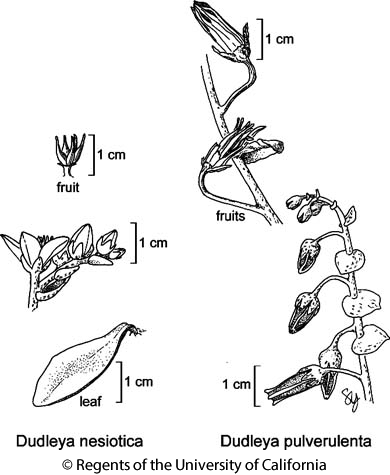
\includegraphics[width=0.6\columnwidth]{figures/fig2-dudleya.png}
\end{center}
\caption{Illustration of \Dudleyanesiotica\ plant \cite{jeps2019dudleya}.}
\label{fig:1.1.2}
\end{figure}






\subsection{Additional Background Research}
We hope to develop innovative methods in the fields of surveying, identification, and object retrieval in places that are difficult to reach. This technology can be refined and tailored for industrial or military in survey and retrieval. 

We looked at the history of air and water temperatures for the environment surrounding the Channel Islands over the past five years during the month of March, our intended operational period. The average air temperature in March has a high of \SI{65}{\fahrenheit} and a low of \SI{49}{\fahrenheit} \cite{accuweather2019channel}. The average water temperature has a high of \SI{58.8}{\fahrenheit} and a low of \SI{53.6}{\fahrenheit} \cite{accuweather2019channel}. In the case where a human person is thrown off the Rigid Hull Inflatable Boat (RHIB) and into the water we have \SIrange{1}{2}{\hour} to rescue them before they develop hypothermia in water conditions from \SIrange{50}{60}{\fahrenheit}. Fog is a common weather feature, especially at San Miguel and Santa Rosa Islands \cite{nps2019weather}. Fog is most common in spring and summer, and west of the Santa Cruz Channel \cite{nps2019weather}. The marine layer fog flows down the coast with the prevailing NW wind, and bends around Point Conception, usually blanketing San Miguel and Santa Rosa, and often the western portion of Santa Cruz Island \cite{nps2019weather}. Fog frequently is thicker and lingers longer into the day offshore than along the mainland coast \cite{nps2019weather}. Preliminary data from Santa Cruz Island suggests that geographic variation in the presence and duration of the fog layer has a profound influence on the temperature and humidity regimes \cite{nps2019weather}. Furthermore, the island chain itself has eight major islands with the largest having an area of \SI{96.51}{\mile\squared} \cite{nps2019weather}. 
\begin{figure}
\begin{center}
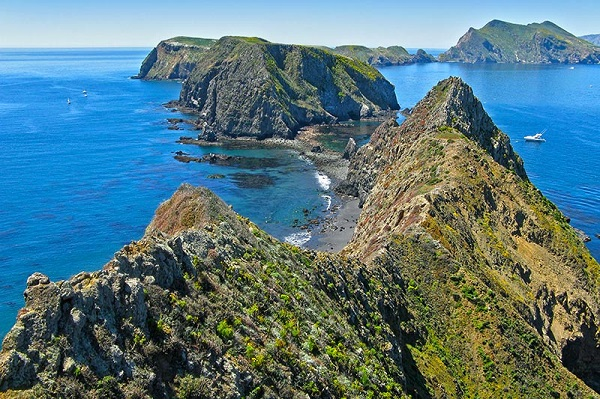
\includegraphics[width=0.8\columnwidth]{figures/fig3-channel.png}
\end{center}
\caption{Aerial Image of the Channel Islands. The larger islands form a National Park which hold many endemic and endangered species of plants \cite{nps2019webpage}.}
\label{fig:1.2.1}
\end{figure}

\begin{figure}
\begin{center}
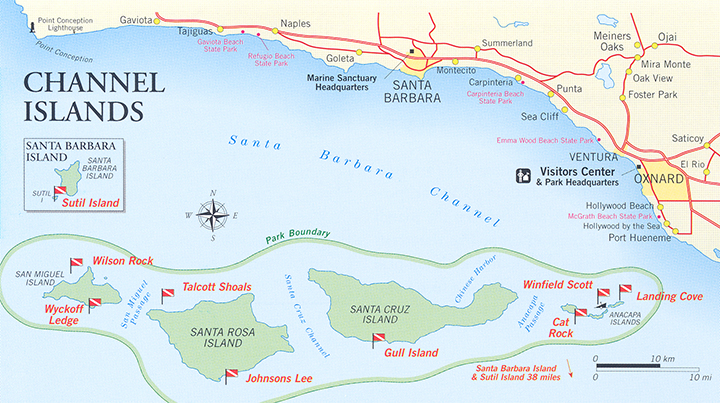
\includegraphics[width=0.8\columnwidth]{figures/fig4-map.png}
\end{center}
\caption{Map of the Channel Islands National Park located 30 miles South of the Santa Barbara Coast \cite{nps2019submerged}.}
\label{fig:1.2.2}
\end{figure}






\section{Problem Statement}
\subsection{Problem Statement}
Our goal is to support the research of Dr. Matthew Guilliams, plant systematist and curator at the Santa Barbara Botanical Garden's Clifton Smith Herbarium, through the survey, extraction, and recovery of the \Dudleyanesiotica\ and \Malvaassurgentiflora, plants endemic to the Channel Islands. Operations will take place near the coastal cliffs of the Channel Islands located off the coast of Santa Barbara. These remote islands are accessible only by boat, and by law, humans are forbidden to step foot on certain islands for environmental protection measures. The two plants of interest are in the vicinity of possibly endangered species, so the team must not harm or disturb the plants surrounding the plant of interest. 

\subsection{Functions}
\begin{figure}
\begin{center}
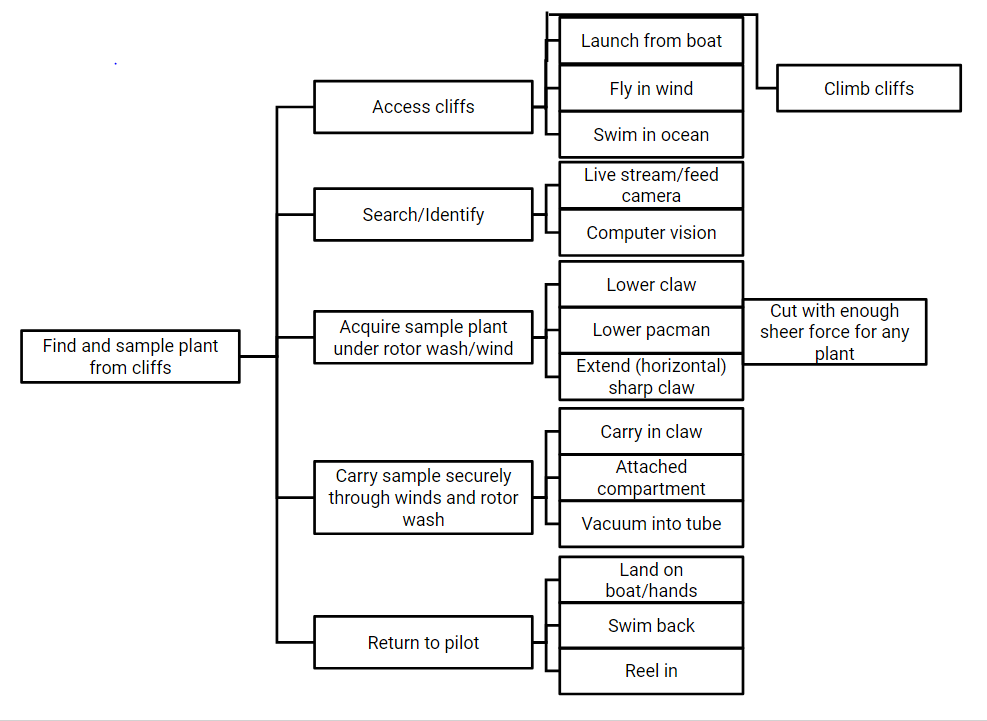
\includegraphics[width=\columnwidth]{figures/fig5-function-tree.png}
\end{center}
\caption{Function Means Tree of the System}
\label{fig:2.2.1}
\end{figure}

\subsection{Constraints}
The average air temperature of the Channel Islands in March is a high of \SI{65}{\fahrenheit} and a low of \SI{49}{\fahrenheit} \cite{accuweather2019channel}. Colder air temperatures will affect the gear needed for operations such as the need for layered clothing, gloves, and thermal insulators for UAS batteries. The average water temperature in March can range from a high of \SI{58.8}{\fahrenheit} and a low of \SI{53.6}{\fahrenheit} \cite{nps2019weather}. If water temperatures are low and the air temperatures are high, there is a high chance for fog which may potentially decrease the field of vision. Severe fog will affect vision and could lead to modification or cancellation of UAS operations. If water temperatures are high, there may be an increase in humidity that will affect the UAS system. Safety during UAS operations are a top priority, thus we must follow safety protocol to ensure no one in the team is at risk for injury or death. As sea state is another factor that will affect RHIB operations, the UAS operations must be done in Channel Island locations with low sea state conditions to ensure optimal operational success. The operational environment is different from a typical flat ground environment in which the Channel Islands’ geography is full of rugged terrain and cliffs. The plants of interest are usually found along the slanted cliffs of the islands, thus we must take into consideration of how the UAS will be designed to ensure the best chances of success in extracting and securing plant samples. 

The landing platform for the UAS operations will be conducted from a RHIB. There will be a limited amount of space for takeoff and landing. There will need to be room for the whole group (five personnel) and a botanist/scientist.  The system must be capable of VTOL (Vertical Takeoff and Landing). In terms of the time period for operation, UAS operations must be conducted during daylight. If there is a day where we cannot fly, there is no way to make up the time by flying at night. The UAS operation cannot damage the environment or other species as the species may be endangered. If the operations were to fail, we must make sure that the UAS will not crash into the island and destroy nature.  Also, one must know when extracting a sample is the appropriate action. For safety of team during RHIB operations, UAS take off, and UAS landing, since the UAS will be taking off and landing on the RHIB, we must make sure that we create and practice a specific and reliable procedure. A constraint concerning securing sample is when the UAS is returning to RHIB, it can be difficult with rotor wash and wind. 

\subsection{Objectives, Pairwise Comparison Chart, and Weightings} 
\begin{table}
\caption{Objective Table split into two portions: mobility and extraction. Objectives for Mobility portion: Part of the system that makes the plant accessible}
\label{tab:2.4.1}
\begin{center}
%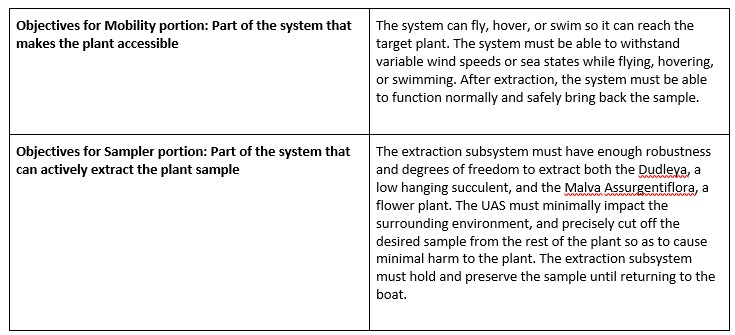
\includegraphics[width=\columnwidth]{figures/table-241.jpg}
\begin{tabular}{p{0.5\columnwidth}p{0.5\columnwidth}}
\toprule
Objectives for Mobility portion: Part of the system that makes the plant accessible &% 
The system can fly, hover, or swim so it can reach the target plant. The system must be able to withstand variable wind speeds or sea states while flying, hovering, or swimming. After extraction, the system must be able to function normally and safely bring back the sample. \\
Objectives for Sampler portion: Part of the system that can actively extract the plant sample &%
The extraction subsystem must have enough robustness and degrees of freedom to extract both the \Dudleya, a low hanging succulent, and the \Malvaassurgentiflora, a flower plant. The UAS must minimally impact the surrounding environment, and precisely cut off the desired sample from the rest of the plant so as to cause minimal harm to the plant. The extraction subsystem must hold and preserve the sample until returning to the boat. \\
\bottomrule
\end{tabular}
\end{center}
\end{table}

The system can fly, hover, or swim so it can reach the target plant. The system must be able to withstand variable wind speeds or sea states while flying, hovering, or swimming. After extraction, the system must be able to function normally and safely bring back the sample.

Objectives for Sampler portion: Part of the system that can actively extract the plant sample
The extraction subsystem must have enough robustness and degrees of freedom to extract both the \Dudleya, a low hanging succulent, and the \Malvaassurgentiflora, a flower plant. The UAS must minimally impact the surrounding environment, and precisely cut off the desired sample from the rest of the plant so as to cause minimal harm to the plant. The extraction subsystem must hold and preserve the sample until returning to the boat.
\begin{table}
\caption{Pairwise Comparison Chart: each metric was compared to the other metrics to determine weights of each metric based on importance to the system.}
\label{tab:2.4.2}
\begin{center}
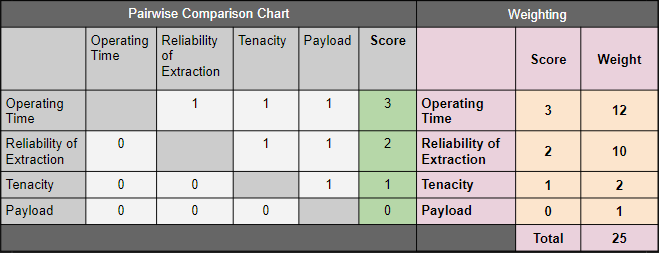
\includegraphics[width=\columnwidth]{figures/table-242.png}
\end{center}
\end{table}



\subsection{Metrics}
Our team developed four metrics to accurately evaluate our design. The metrics are Operating Time, Reliability of extraction, Tenacity, and Total Required Payload. The most important of these metrics is Operating Time since all other metrics depend on the devices ability to successfully operate. Reliability of extraction is the next most important metric since sample extraction is our primary mission.  Tenacity is the third metric due to the environmental factors that must be overcome to accomplish our mission. Lastly our device must have a Payload large enough to support mission necessary equipment.
\begin{table}
\caption{Operating Time Metrics Table}
\label{tab:2.5.1}
\begin{center}
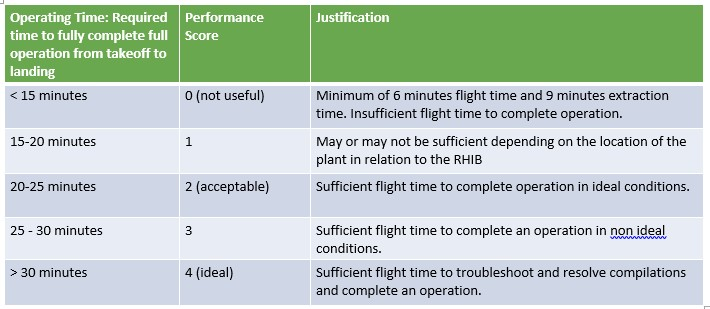
\includegraphics[width=\columnwidth]{figures/table-251.jpg}
\end{center}
\end{table}
\begin{table}
\caption{Reliability of Extraction Metrics Table}
\label{tab:2.5.2}
\begin{center}
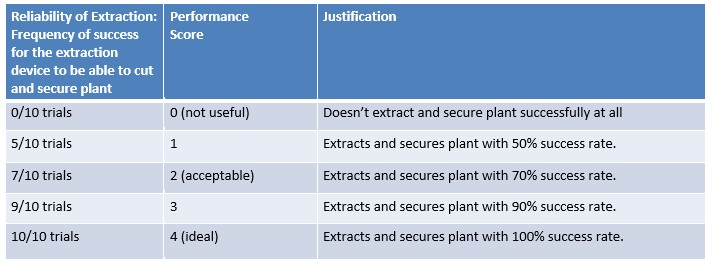
\includegraphics[width=\columnwidth]{figures/table-252.jpg}
\end{center}
\end{table}
\begin{table}
\caption{Total Required Payload Metrics Table}
\label{tab:2.5.3}
\begin{center}
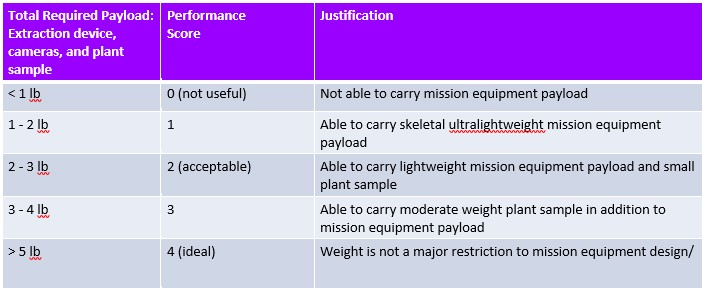
\includegraphics[width=\columnwidth]{figures/table-253.jpg}
\end{center}
\end{table}
\begin{table}
\caption{Tenacity Metrics Table}
\label{tab:2.5.4}
\begin{center}
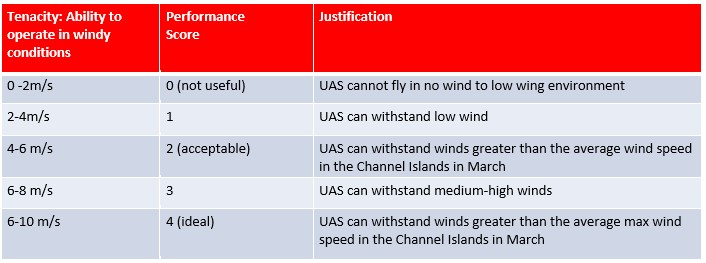
\includegraphics[width=\columnwidth]{figures/table-254.jpg}
\end{center}
\end{table} 






\section{Related Work}
\subsection{National Botanical Garden (NTBG) Plant Survey using UAS}
Ben Nyberg, a UAS operator with NTBG used his UAS to survey and gather footage of plants that are native to Hawaii in hard-to-reach areas.  His job consisted of driving/hiking/helicoptering to the flight location and deploying his UAS.  The average flight time for the UAS ranged from \SIrange{20}{30}{\minute}.  There is usually an assistant with him to help keep the UAS in sight at all times.  All plants are manually identified by the pilot himself during flight operations, and the footage was brought back to other plant experts afterwards.  A big problem that the team ran into was weather.  The islands were very humid and any sort of wind would affect the flight and the control of the UAS \cite{mongabay2019hunting}. 
\begin{figure}
\caption{Picture of Ben Nyberg, a UAS operator with NTBG, using a UAS for surveying \cite{mongabay2019hunting}.}
\label{fig:3.1}
\begin{center}
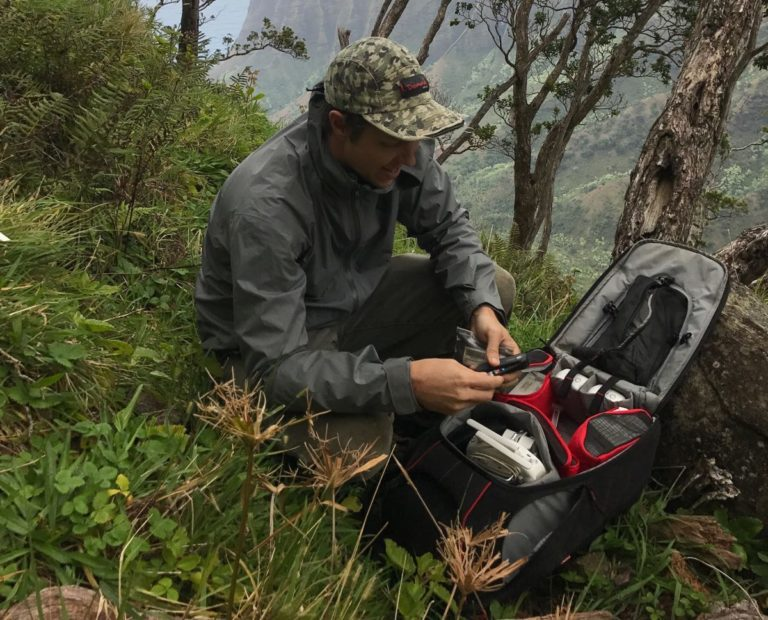
\includegraphics[width=0.8\columnwidth]{figures/fig31-nyberg.png}
\end{center}
\end{figure}

The difference with this design with regards to our mission is that the UAS does not collect samples of the plant and is only used as a means to survey the land. If a species is identified, a professional climber would be airlifted from a helicopter to manually collect the sample. Furthermore, the UAS pilot is able to operate on land where as in our project we will be confined in a RHIB. 

In our design, we would like to create a UAS that can survey the land to identify the desired plants and sample them so that samples do not have to be retrieved manually.  We are also trying to attach additional batteries to our UAS so that the flight time will be increased. A key takeaway from Ben Nyberg’s research is how his team was able to overcome environmental disturbances and compare similarities to that of the Channel Islands. 

\subsection{University of California, Santa Barbara Sampler UAS}
A capstone project of the Mechanical Engineering department of the University of California, Santa Barbara, created a UAS that can fly and take samples of plants.  Their main problem to solve was taking samples of plants in hard-to-reach places using an arm that dangled below the UAS.  The main plants that were sampled were branches of tall trees.  The design that was used can be seen below.
\begin{figure}
\caption{UCSB design for sampler UAS \cite{dantonio2018sampler}.}
\label{fig:3.2}
\begin{center}
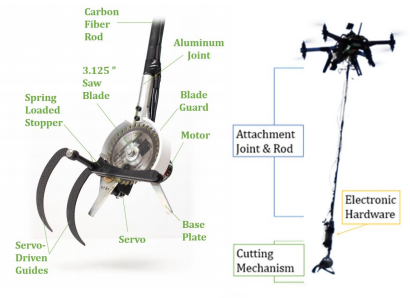
\includegraphics[width=0.8\columnwidth]{figures/fig32-ucsb.png}
\end{center}
\end{figure}

Issues with this design with regards to our mission: Average flight time of \SI{7}{\minute}; Made to cut larger branches; The control of the UAS greatly affected the quality of the sample; Octocopter was used instead of a quadcopter.

Although a working design, the UCSB capstone design was unable to fly for our minimum flight time of \SI{15}{\minute}.  The design also is not ideal for sampling plants that are growing on near-vertical cliffs because the UAS would not be able to position itself directly overhead of the plant. 

\subsection{Airborne refueling probe basket}
The military uses a system called a probe-and-drogue which employs a hose from a tanker aircraft with a drogue (a funnel-like basket) attached to the end of the hose in order to catch the probe on the receiving aircraft.  The basket is made to be drag-resistant and sturdy enough to guide the probe into the nozzle \cite{ren2019reliable}.    
\begin{figure}
\caption{Picture of Airborne refueling probe basket \cite{ren2019reliable}}
\label{fig:3.3}
\begin{center}
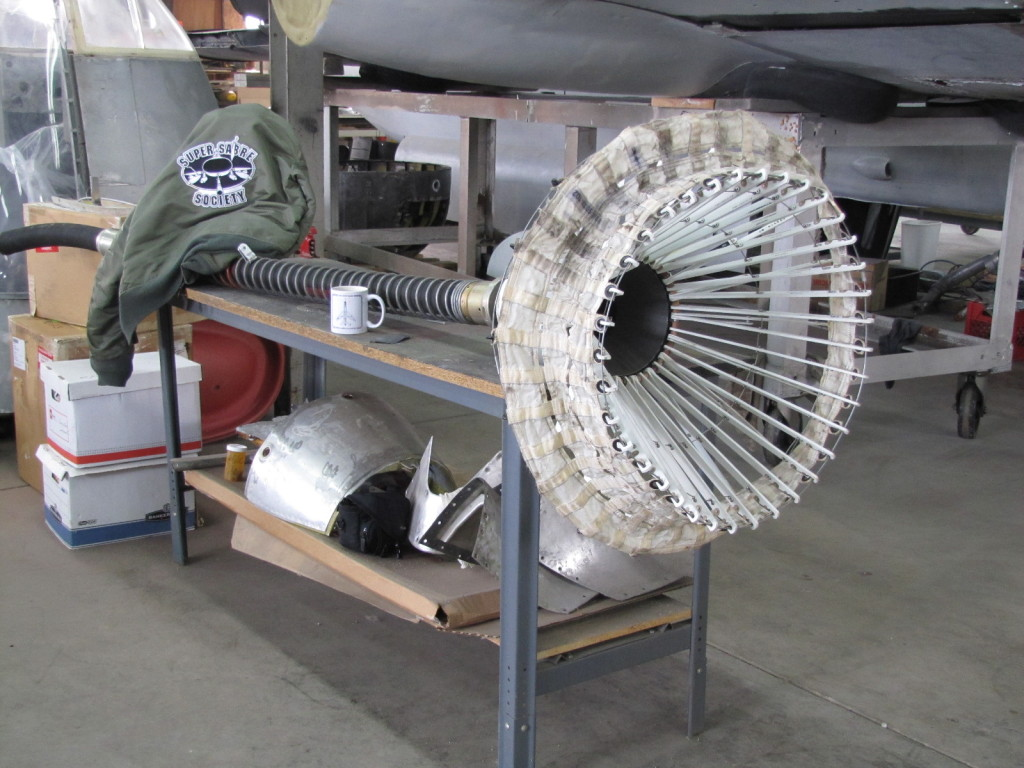
\includegraphics[width=0.8\columnwidth]{figures/fig33-refueling.png}
\end{center}
\end{figure}

This type of design is helpful for the snipper/gripper design because this will help guide the plant into the hole where it can be cut and stored.  However, funneling a plant is different than guiding a fuelling probe.  The refuelling drogue is made to fly backwards while our fixture is facing into the direction of flight.  In our design we incorporated a cone-shaped mesh to help funnel a branch into the cutting zone.





\section{Conceptual Designs}
When reviewing the customer requirements and overall objectives our team was able to derive definitive functions for our conceptual  designs. Overall we want to develop an unmanned UAS system that is able to survey an island, search and identify a species of plant and recover with minimal interference to the plant themselves. Circled red on our morth chart are viable solutions to respective functions. The conceptual design below integrate technologies annotated in the morph chart.
\begin{table}
\caption{Overall Morth Chart with all viable capabilities}
\label{tab:4.1}
\begin{center}
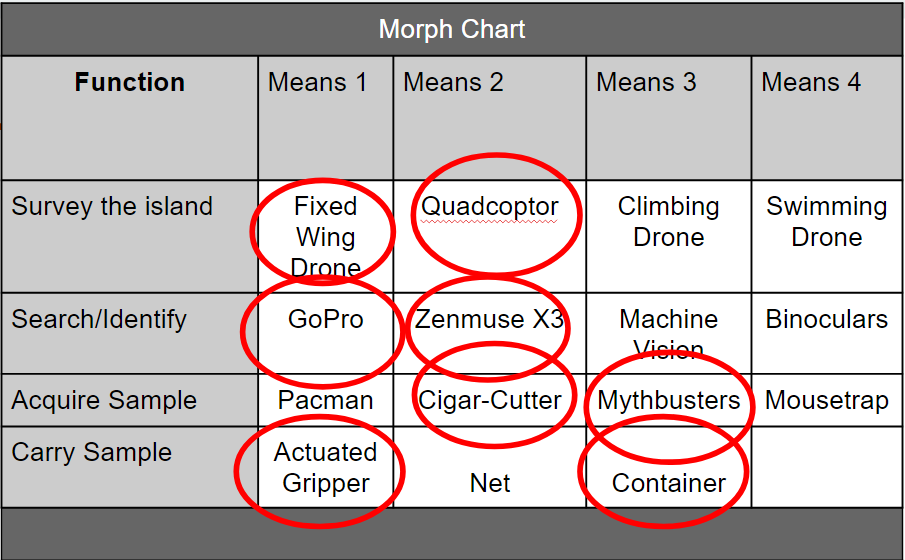
\includegraphics[width=\columnwidth]{figures/table-41.png}
\end{center}
\end{table}


\subsection{Concept 1: Quadcopter Survey and Extraction}
The first concept that was evaluated was the Quadcopter Survey and Extraction. The UAS will only have a camera system when surveying to maximised flight time. Currently we are working with the DJI Matrice 100 and the Zenmuse X3 camera and gimbal \cite{dji2019zenmuse}.  The maximum hovering time of with two batteries, gimbal and camera set up is \SI{30}{\minute} giving us a 3/4 on our operating time matrics \cite{dji2019dji}. \SI{30}{\minute} gives sufficient flight time to complete an operation in non ideal conditions as well as flexibility when surveying island cliffs. While \SI{30}{\minute} is not much time, it's on average higher than other quadcopters of its size and capability. Furthermore the Matrice 100 is able to fly in a maximum of \SI{22}{\mph} wind conditions \cite{dji2016m100}.

With the maximum winds of the Channel Islands in March being \SI{18}{\mph} this system scored a 4/4 on our tenacity metric.  After launching from the RHIB, the UAS will follow waypoints around the perimeter of the island and utilize a camera system to record the cliffside. Once sufficient video is taken or a low power mode is activated the UAS will return back to the RHIB where our team will extract the footage for review.  After reviewing the footage if there is a plant species that needs to be collected we will attach, in addition to the Zenmuse X3 gimbal, our extraction system. 

The Matrice 100 has an estimated maximum payload of \SI{1.15}{\kilo\gram} for one battery excluding the weight of that battery. The maximum weight for two batteries needs to be tested given the extra battery weighs \SI{672}{\gram}. Currently we give the Matrice a  2/4 acceptable rating in our total required payload metric which includes extraction device, camera and plant sample. The Zenmuse X3 and gimbal’s weight is \SI{247}{\gram} giving our team the remander \SI{868}{\gram} to work with. We will release the Matrice, use the extraction system to collect a sample of the plant and return back to the RHIB successfully. The conceptual design of the extractors will be discussed later in this section.  
\begin{figure}
\begin{center}
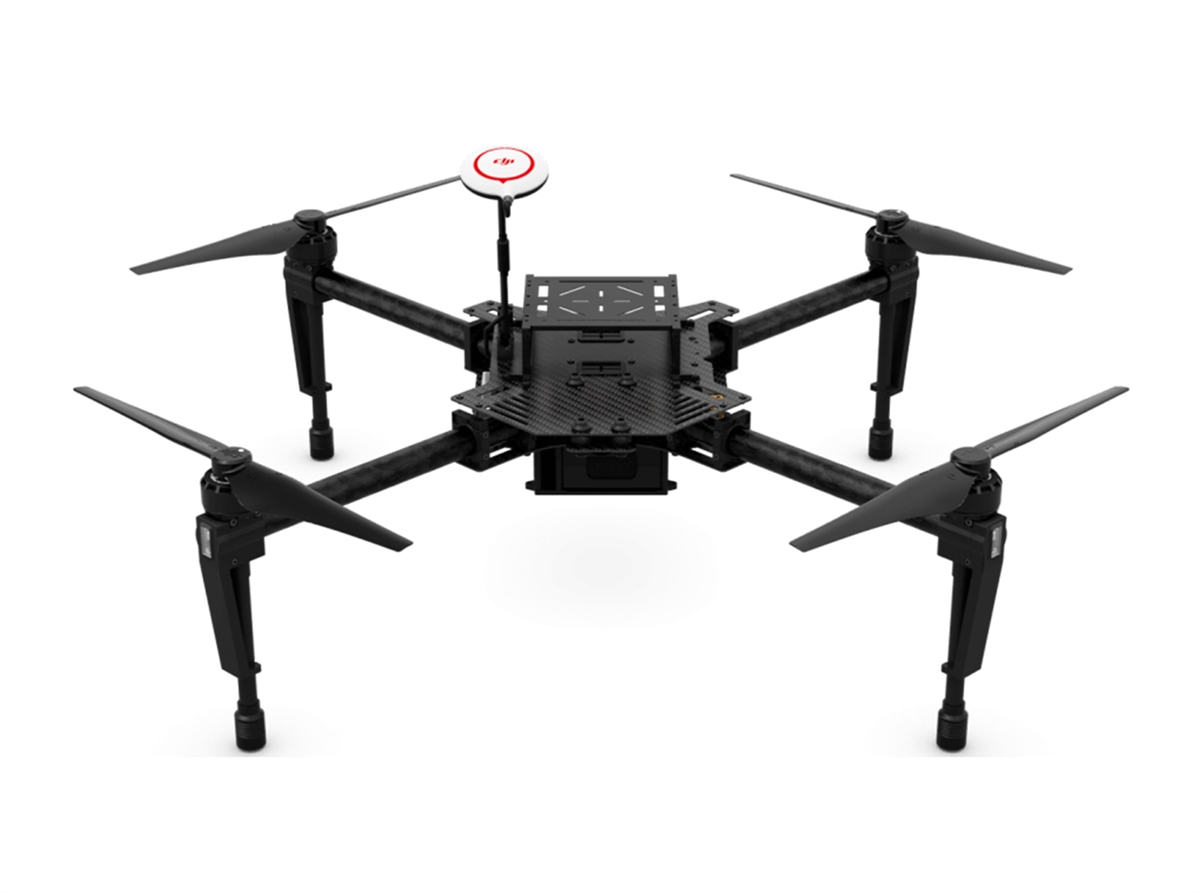
\includegraphics[height=1.3in]{figures/fig411a.png}
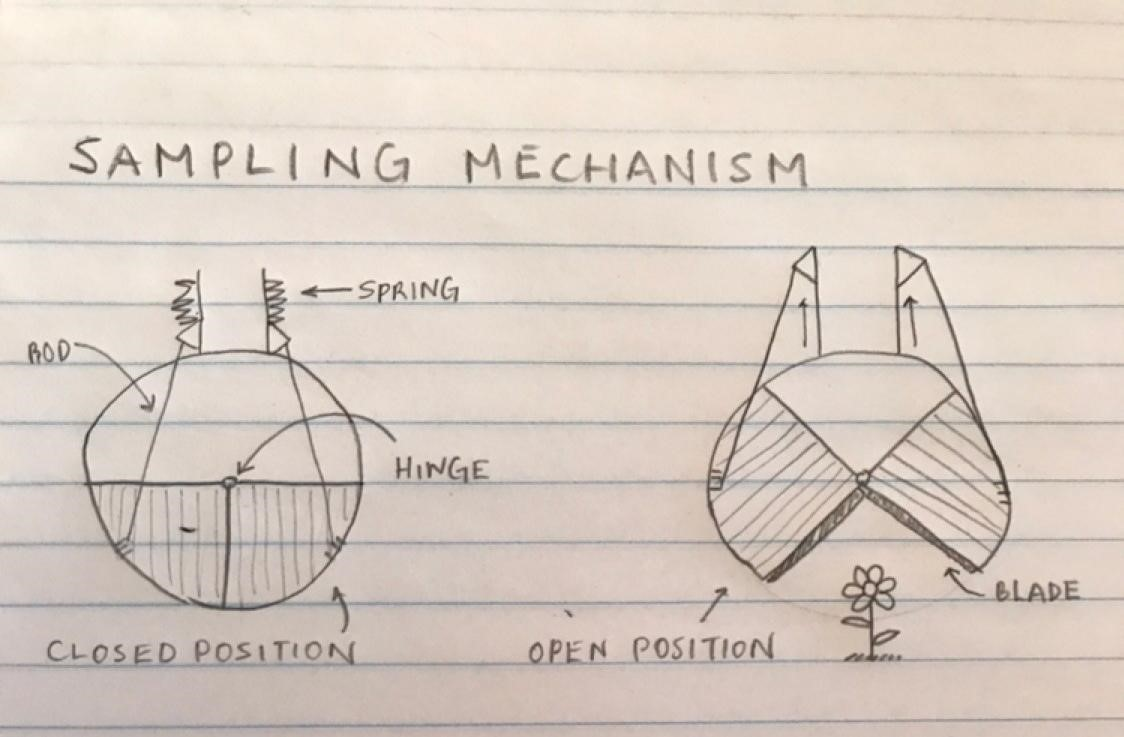
\includegraphics[height=1.3in]{figures/fig411b.jpg}
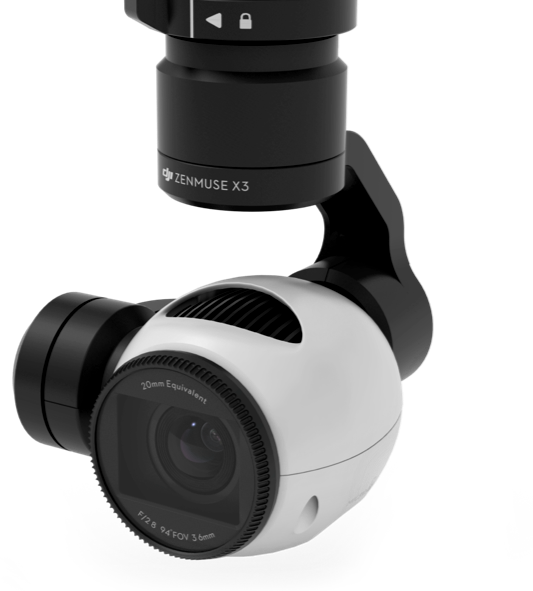
\includegraphics[height=1in]{figures/fig411c.png}
\end{center}
\caption{DJI Matrice 100, Prototype Drawing of Extraction Mechanism, and Zenmuse X3 Gimbal respectively \cite{dronesmadeeasy2019matrice, dji2019zenmuse}.}
\label{fig:4.1.1}
\end{figure}



\subsection{Concept 2:  Fixed-Wing Quadrotor Combo}
The second concept that was evaluated was the Fixed-Wing Quadrotor Combo. The Fixed Wing UAS would be used for the initial steps of surveying the island to search and identify the respective plant species. On average the operating time of fixed wing aerial systems is \SI{45}{\minute} giving the Operating Time metric a 4/4. \SI{45}{\minute} gives sufficient time to troubleshoot complications if arise and complete the operation. The payload of the Fixed Wing UAS is not as important because there are usually built in cameras. Whereas the payload and overall specifications of the Quadcopter will be the same as in concept one. The Matrice 100  would be sent out to desired plant location for extraction due to its higher stability. The pros of incorporating the fixed wing UAS would be an estimated 50\% increase in operating time and potentially high video quality. The downside would be purchasing/acquiring a whole new system, learning how to use it and takeoff/landing procedures. We looked at the WingtraOne, a fixed wing UAS developed by Wingtra \cite{wingtra2019wingtraone}. The Wingtra has no listed price but camera offers a minimal ground sampling distance of \SI{0.7}{\centi\meter} and vertical take off and landing \cite{wingtra2019wingtraone}. 

\begin{figure}
\begin{center}
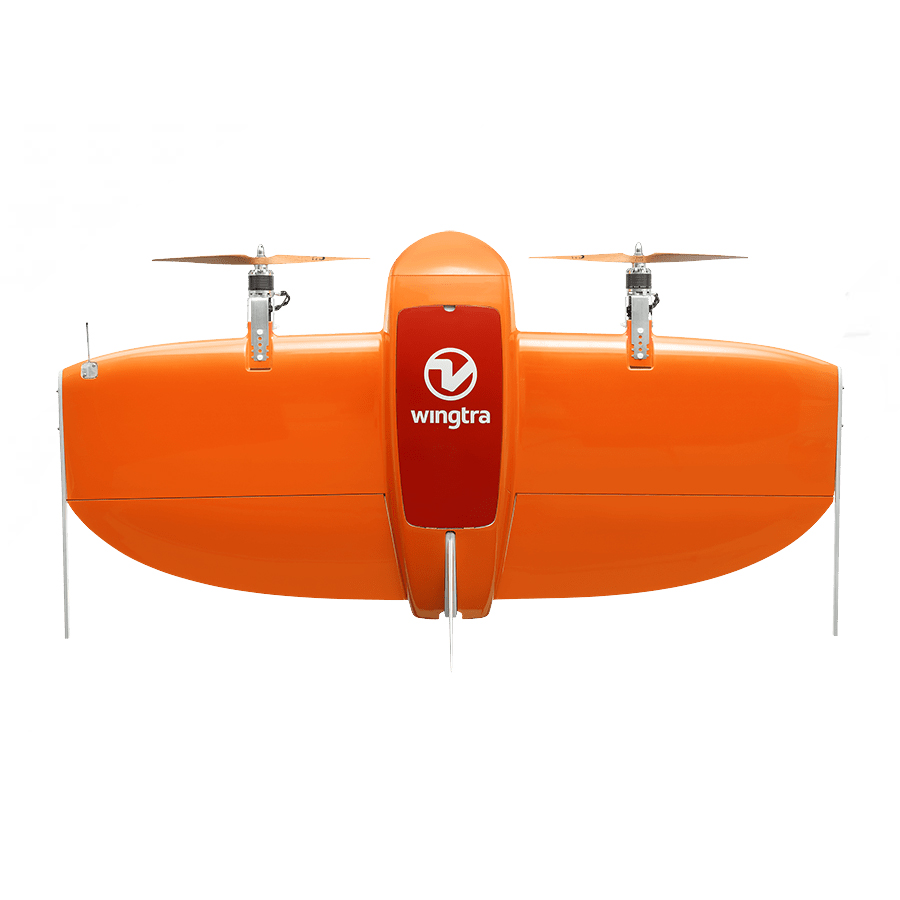
\includegraphics[height=1in]{figures/fig421a.png}
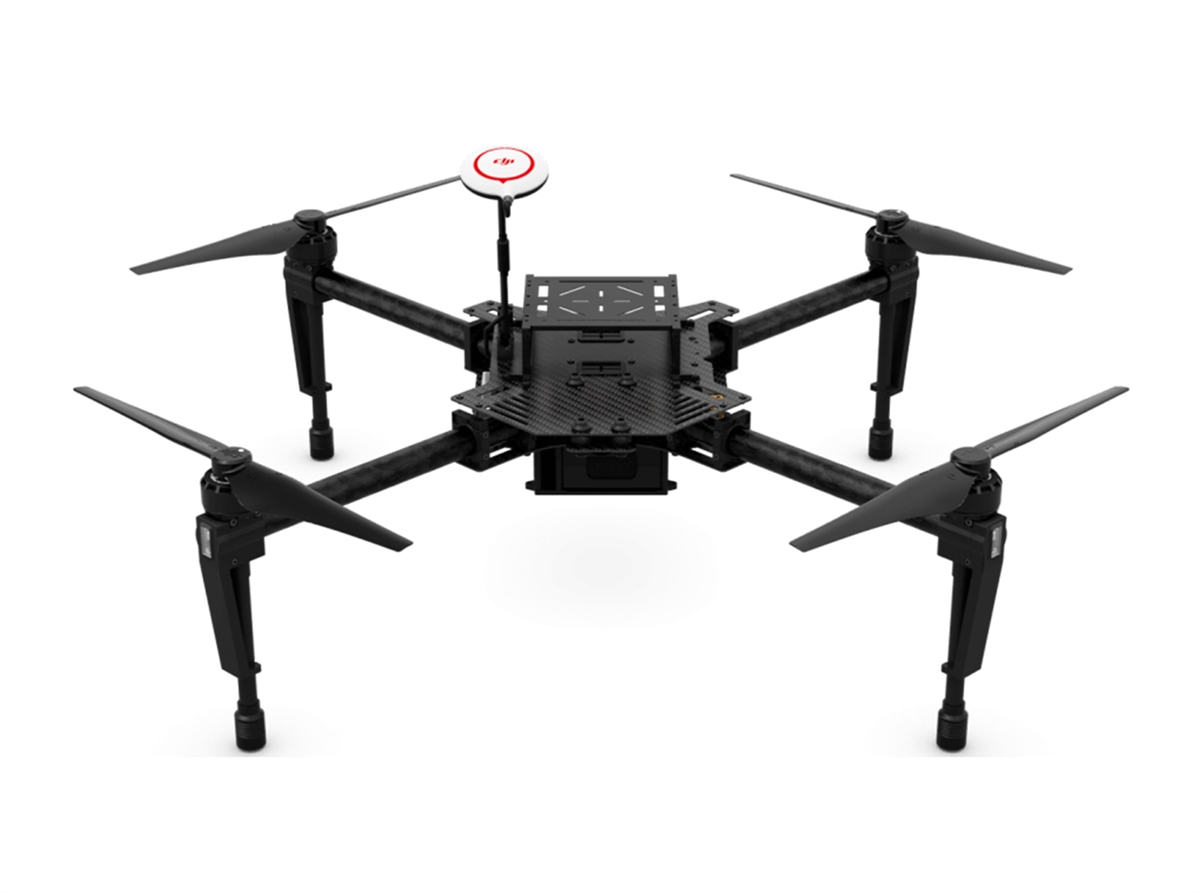
\includegraphics[height=1in]{figures/fig421b2.png}
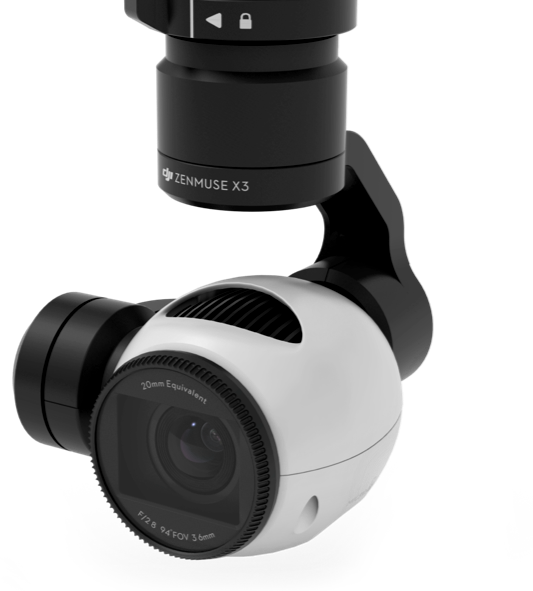
\includegraphics[height=0.2in]{figures/fig421b1.png}
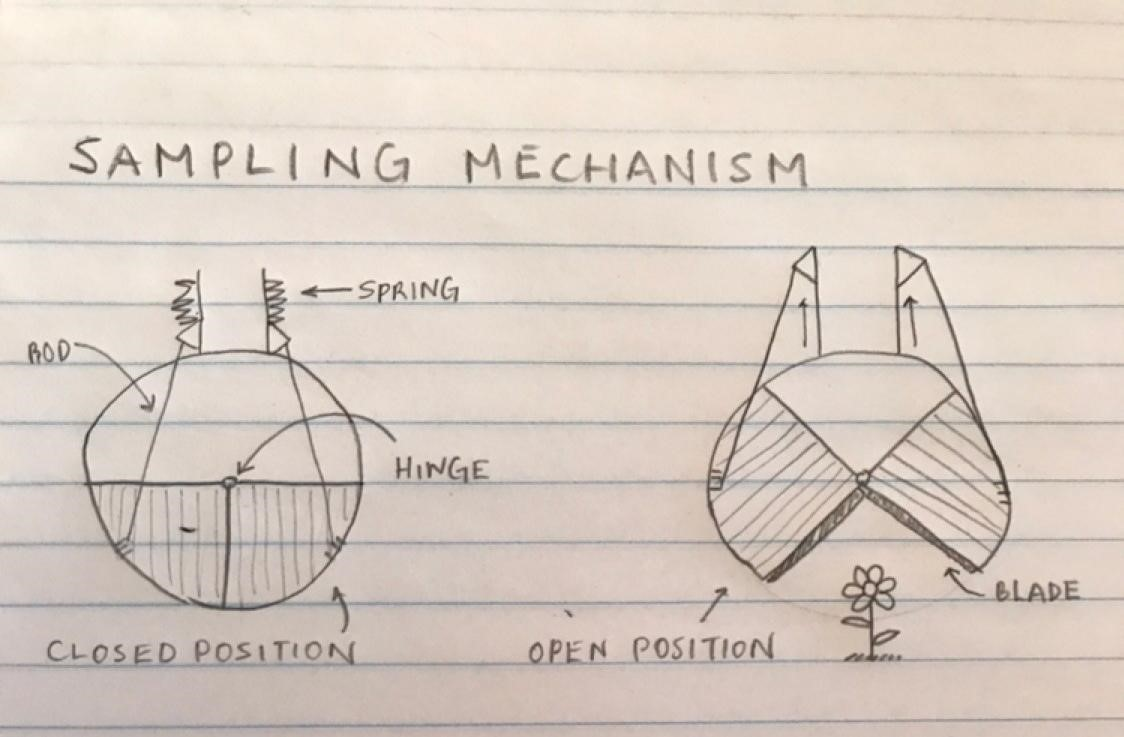
\includegraphics[height=0.8in]{figures/fig421c.jpg}
\end{center}
\caption{Fixed-wing UAS, DJI Matrice 100 with Zenmuse X3 Attached, and Prototype Drawing of Extraction Mechanism respectively  \cite{dronesmadeeasy2019matrice, wingtra2019wingtraone, dji2019zenmuse}}
\label{fig:4.2.1}
\end{figure}





\subsection{Concept 3:  Climbing Robot}
Robot with Four Servo legs that is able to climb onto steep rocky cliffs and be able to extract plant sample through extraction device beneath the robot. The benefits of this design are its operating time, payload and tenacity. The robot itself needs to be transported onto the island via quadcopter. Because the robot is constricted to the ground and limited in movement its use for surveying the island to search and identify plants would be futile. Whereas recovering the plant would not be, given that a ground system does not need to adhere to the same physics as our air counterparts we will be able to attach a hefty payload and in turn maximise our operating time.  Cliff Climbing Robots are built with hook like claws to attach to rocky surfaces and potentially with anti-vibration and anti-wind loading. The robot will be able to withstand the highest winds speed of the channels island scoring highest in our tenacity metric. While  these ideas are great in theory, developing a whole robotic cliff climbing robot is beyond our capabilities  and level of experience. Furthermore, the system that delivers the UAS must provide a payload that can withstand the weight of the robot. 
\begin{figure}
\begin{center}
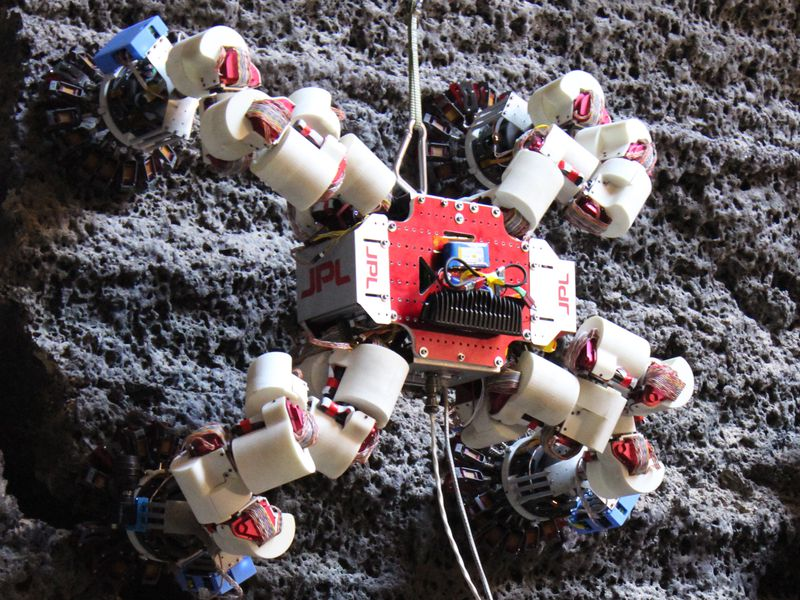
\includegraphics[width=0.5\columnwidth]{figures/fig431.png}
\end{center}
\caption{NASA JPL Lemur 3 Climbing Robot \cite{donahue2017new}}
\label{fig:4.3.1}
\end{figure}



\subsection{Concept 4: Cigar-Cutter Extraction Mechanism}
This extraction system utilizes spring power over a cigar cutter to cut the plant. It is strategically placed behind a cone and before a clear tube so that once the spring mechanism is activated it will not only cut the plant but also trap it in the tube, securing the plant inside the tube for recovery. There will be a camera that points to the clear tube so that the UAS co-pilot will know when to activate spring loaded trap while the main UAS pilot can focus on positioning the UAS during the extraction process. This system is predicted to work 5/10 trials. This is not because the cutter will not cut through  the plant, but the limitation of if the plant does not go into the cone all the way and the spring is activated. Another limitation is that the cigar-cutter is one try method because the cigar cutter cannot be reset unless the UAS returns to the boat and physically reset by hand. 
\begin{figure}
\begin{center}
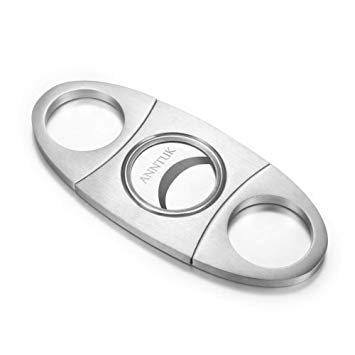
\includegraphics[width=0.5\columnwidth]{figures/fig441.png}
\end{center}
\caption{Sample picture of cigar cutter used for design \cite{famoussmoke2019cigar}}
\label{fig:4.4.1}
\end{figure}





\subsection{Concept 5: Mythbuster Motorized Shear}
Developed by Mythbusters host Jamie Hyneman, the motorized shear uses a high torque motor and a worm drive gear orientation to translate a motor’s single axis spin into planar rotational motion. The planar circular motion controls the end effector shears to repeatedly open and close at a comfortable speed. In the video, Jamie Hyneman demonstrates how powerful the shears are by easily cutting through thick branches, and then proceeds to attach the subsystem to his UAS. He flies the UAS to a bush and begins cutting branches off \cite{mbed2019}. This is exactly the kind of design that we envision.
\begin{figure}
\begin{center}
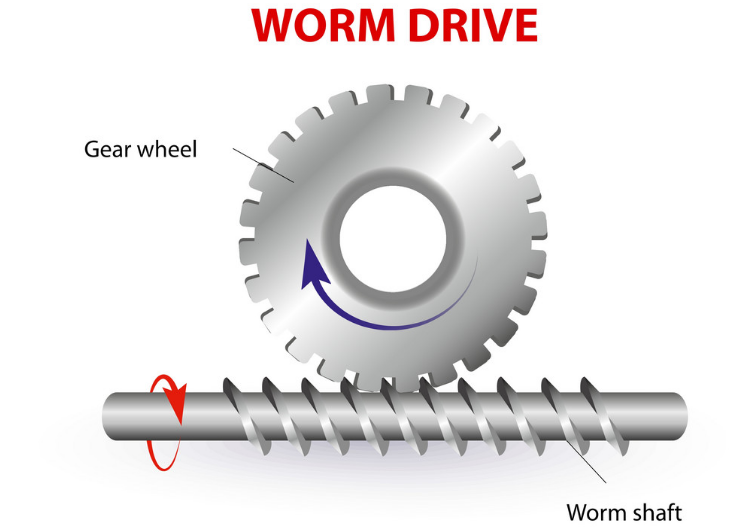
\includegraphics[width=0.5\columnwidth]{figures/fig451.png}
\end{center}
\caption{Worm drive diagram that shows how axis rotation can be translated into rotational planar motion \cite{wikipedia2019wormdrive}.}
\label{fig:4.5.1}
\end{figure}
\begin{figure}
\begin{center}
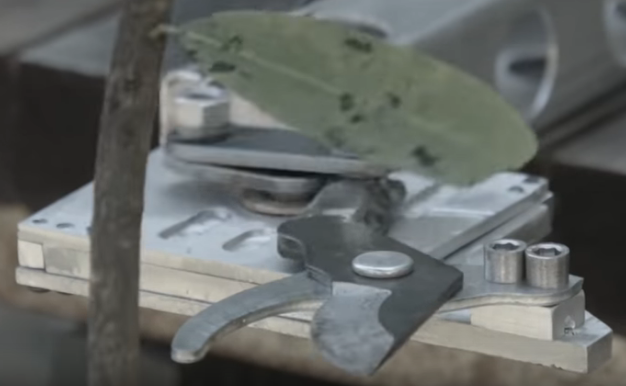
\includegraphics[width=0.4\columnwidth]{figures/fig452.png}
\end{center}
\caption{The end effector of the motorized shear \cite{mbed2019}.}
\label{fig:4.5.2}
\end{figure}







\subsection{Decision Matrix}
\begin{table}
\caption{Decision Matrix Chart}
\label{tab:4.6.1}
\begin{center}
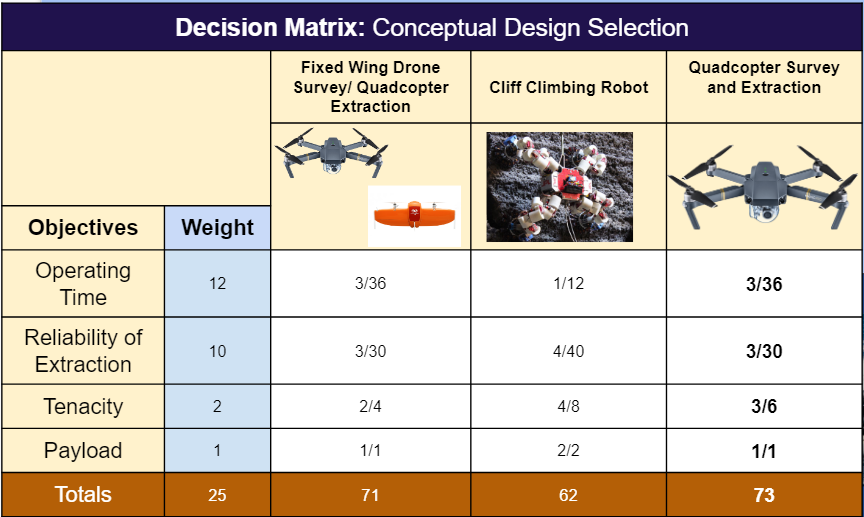
\includegraphics[width=\columnwidth]{figures/table-461.png}
\end{center}
\end{table}

\Fref{tab:4.6.1} shows our analysis of comparing all three he designs. While the single quadcopter design scored the highest, the Fixed Wing UAS Survey with Quadcopter Extraction came in a close second. The only difference in the matrix of these is that the single UAS system is less complex and therefore has less room for failure. The Climbing Robot involves too many additional pieces needed such as a way to send out and retrieve the robot after a successful extraction. We speculate the Climbing Robot to be the most reliable in extraction, but operating a robot from afar on a boat seems much too difficult. Though the single quadcopter design won in terms of points on the decision matrix, our group has still not given up on the idea of a quadcopter and fixed wing project. During the first semester, we focused on the extraction and flying elements of the quadcopter because it is the quadcopter that will ultimately do the extraction. We plan to incorporate testing with a fixed wing UAS for survey purposes.

\begin{figure}
\caption{Functional Block Diagram of the DJI M100 with a Motorized End Effector}
\label{fig:4.6.1}
\begin{center}
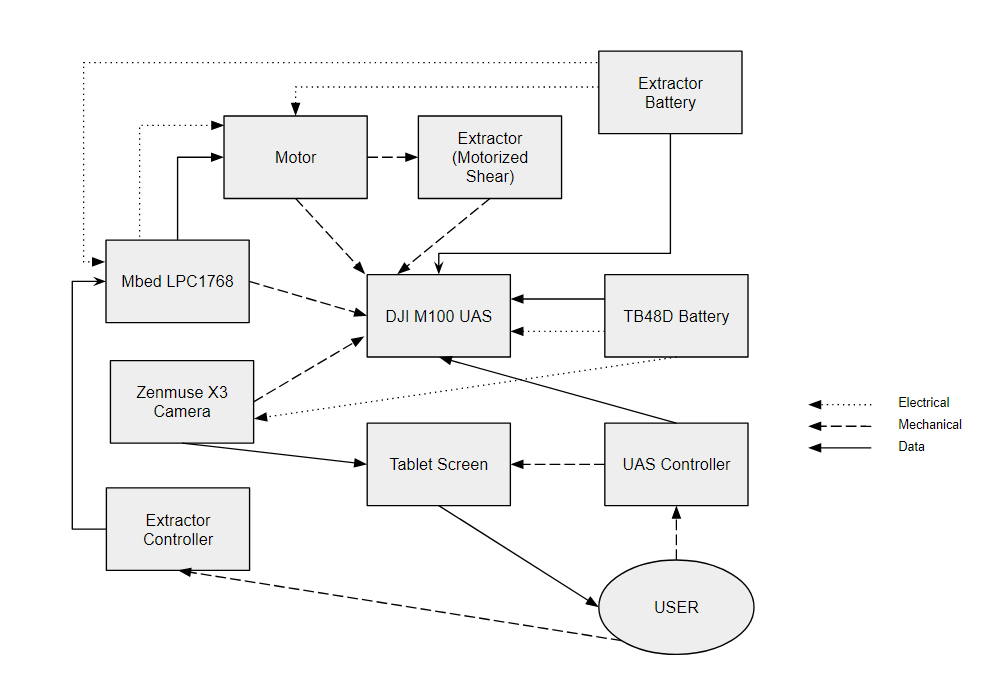
\includegraphics[width=\columnwidth]{figures/fig461.png}
\end{center}
\end{figure}







\section{Ethical Considerations}

Our project inherently contained a lot of space restrictions, and the nature of the mission has many restrictions placed by the Environmental Protection Agency (EPA).  A primary ethical concern for our project is nested in the act of damaging endangered species.  In order to retrieve a sample of an endangered species, it must be damaged.  This goes against the Endangered Species Act (ESA) of 1973 which states that endangered species cannot be carried, delivered, received, or shipped \cite{czech2001endangered}.  The act also states that endangered species cannot be damaged or destroyed in knowing violation of any law.  The Santa Barbara Botanical Garden has a permit to invade these islands and collect the samples.  As a team, we must make sure that, even though we have permission to damage the endangered plant life, we keep the damage to a bare minimum.  As a team, we must make sure that the assurances we make are honest and realistic to ensure that there is no miscommunication of expectations between us and the customer (for example: if our system is likely to damage to  the plant and the surrounding cliff, we must be clear about it).  This complies with the Institute of Electrical and Electronics Engineers (IEEE) Code of Ethics.  During testing, there may be times when we are forced to make a decision between the safety of ourselves or the safety/success of the mission.  For example, when landing the drone on the boat, team members may reach out to grab the drone if it looks like it will not stably land on the platform.  This may potentially cause the team member to hurt his/her hand or fall out of the boat.  As a team, we must comply with the IEEE Code of ethics which states that we need to ``hold paramount the safety of the public'' and ``avoid injuring others.''  In order to mitigate this risk, we must understand our own capabilities and only attempt endeavors at which we are most likely to succeed.  Being aware of one’s capabilities and acting within our abilities is emphasized by both the IEEE Code of ethics, and the Profession Engineer’s Code. 





\section{Engineering Standards and Specifications}

\begin{table}
\caption{Lithium Battery Standards Table \cite{mpoweruk2019international}}
\label{tab:6.1}
\begin{center}
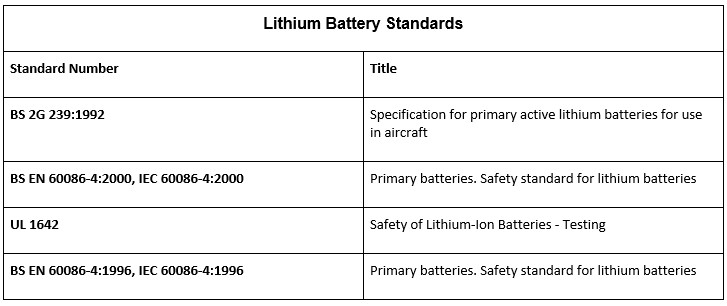
\includegraphics[width=\columnwidth]{figures/table-61.jpg}
\end{center}
\end{table}

Lithium Batteries are a staple in any operation involving UAS because of their high specific energy, extremely advantageous when weight is a constraint. There are numerous standards for lithium polymer battery training, safety, and use in aircraft operations. Our team completed lithium polymer battery training with Professor Evangelista.






\section{Preliminary Detailed Design}
\subsection{Component Selection}
The UAS system we chose to use was the DJI Matrice 100. In respect to our design matrix of ``operating time'' the Matrice 100 offeres us a performance score of acceptable (2/4) providing sufficient time (\SIrange{20}{25}{\minute}) to complete operation in ideal conditions.  We determined the acceptable operating time of \SIrange{20}{25}{\minute} from reviewing the DJI Matrice 100 manual, available battery power of the TD48B smart Batteries and estimated overall payload. The DJI Matrice 100 also satisfies another design matrix ``Total Required Payload'' with a score of acceptable (2/4) being able to carry lightweight mission equipment payload and small plant sample. We determined that the total weight of our payload to include snipper/gripper, attachment system, camera, gimbal and external power should not weigh more than \SIrange{2}{3}{\pound}. Furthermore the DJI Matrice 100 satisfies another design matrice ``tenacity'' the ability to operate in windy conditions with a performance score of acceptable (2/4) able to overcome \SIrange{4}{6}{\meter\per\second} which are greater than average wind speed in the Channel Islands in March.  The camera system we chose to use is the Zenmuse X3. We chose the Zenmuse X3 for our beginning stages of prototyping because it provides us with an extremely user accessible gimbal. The controllable range is tilt \ang{+30} to \ang{-90}, pan \ang{\pm 320} and roll of \ang{\pm 15}. The camera quality itself is descent with 12 megapixels of resolution and $\num{3.5}\times$ zoom. It is able to record at a maximum UDH 4k 25p and has a white balance option for cloudy conditions. Furthermore it has the capacity to store up to 64 gb on a mini SD card. 
        
\subsection{Parts List and Budget}
\begin{table}
\caption{Complete Parts List}
\label{tab:7.2.1}
\begin{center}
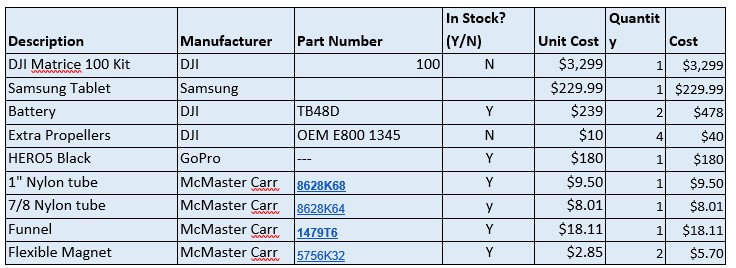
\includegraphics[width=\columnwidth]{figures/table-721.jpg}
\end{center}
\end{table}
\begin{table}
\caption{Complete Budget List. Disclaimer: ``labor'' costs and person-day rates are solely for EW401 training purposes and do not reflect actual costs.}
\label{tab:7.2.2}
\begin{center}
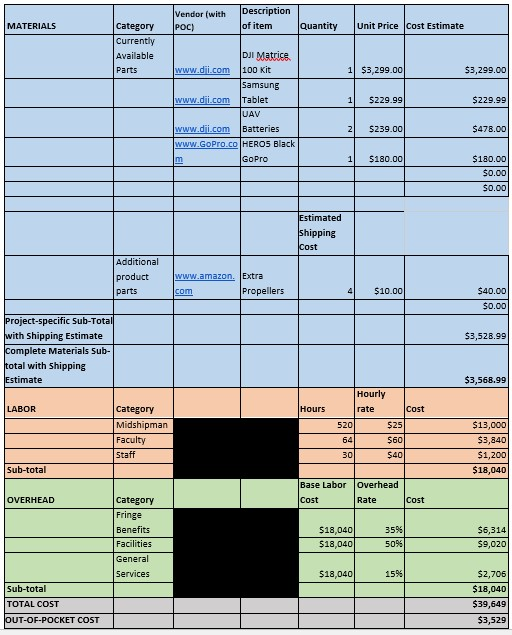
\includegraphics[width=\columnwidth]{figures/table-722.jpg}
\end{center}
\end{table}





\subsection{Mechanical Drawings}

\begin{figure}
\begin{center}
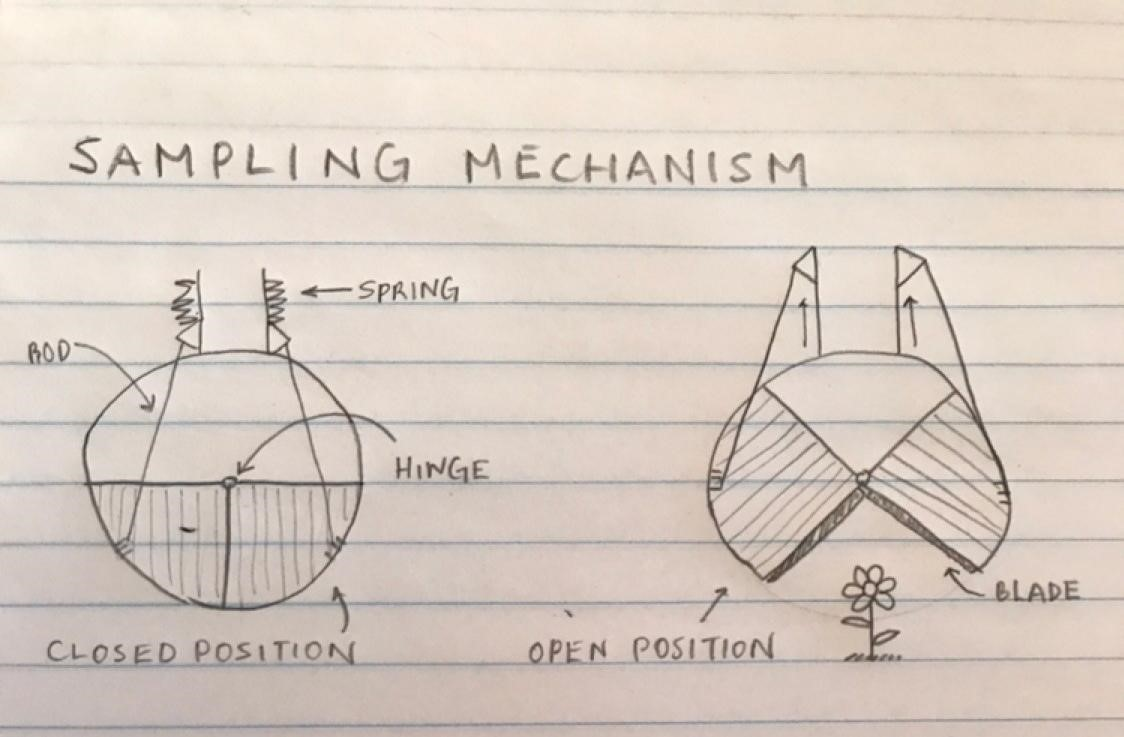
\includegraphics[width=0.8\columnwidth]{figures/fig731.jpg}
\end{center}
\caption{A prototype drawing of the initial Pac-Man design for extraction}
\label{fig:7.3.1}
\end{figure}
Initially, a grabber system that resembled a video game character, Pac-Man, was contemplated.  The apparatus would be attached to the end of a long rod attached to the UAS, and actuated by a solenoid.  The design incorporated blades on the sliding hatches that were pushed closed by strong springs that were attached to the rod portion.  For simplicity, and conservation of weight, the design was a strong, single-cut (one and done). 

After some rumination, the Pac-Man design was altered in order to have less moving parts.  The second design looked more like the mouth of an eel.  Unlike the two moving hatches of the initial design, the new grabber system was designed with a fixed bottom jaw which would act like an anvil to the blade attached to the top jaw.  The top jaw would be snapped closed using tension from strong torsion springs similar to those found in a household mousetrap.
\begin{figure}
\begin{center}
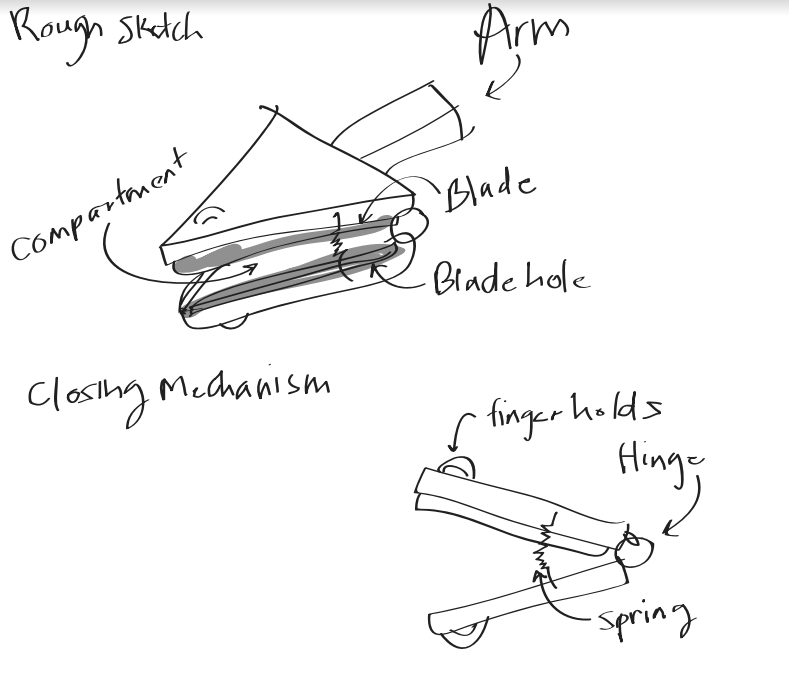
\includegraphics[width=0.6\columnwidth]{figures/fig732.png}
\end{center}
\caption{A rough sketch of the revised Pac-Man design}
\label{fig:7.3.2}
\end{figure}

\begin{figure}
\begin{center}
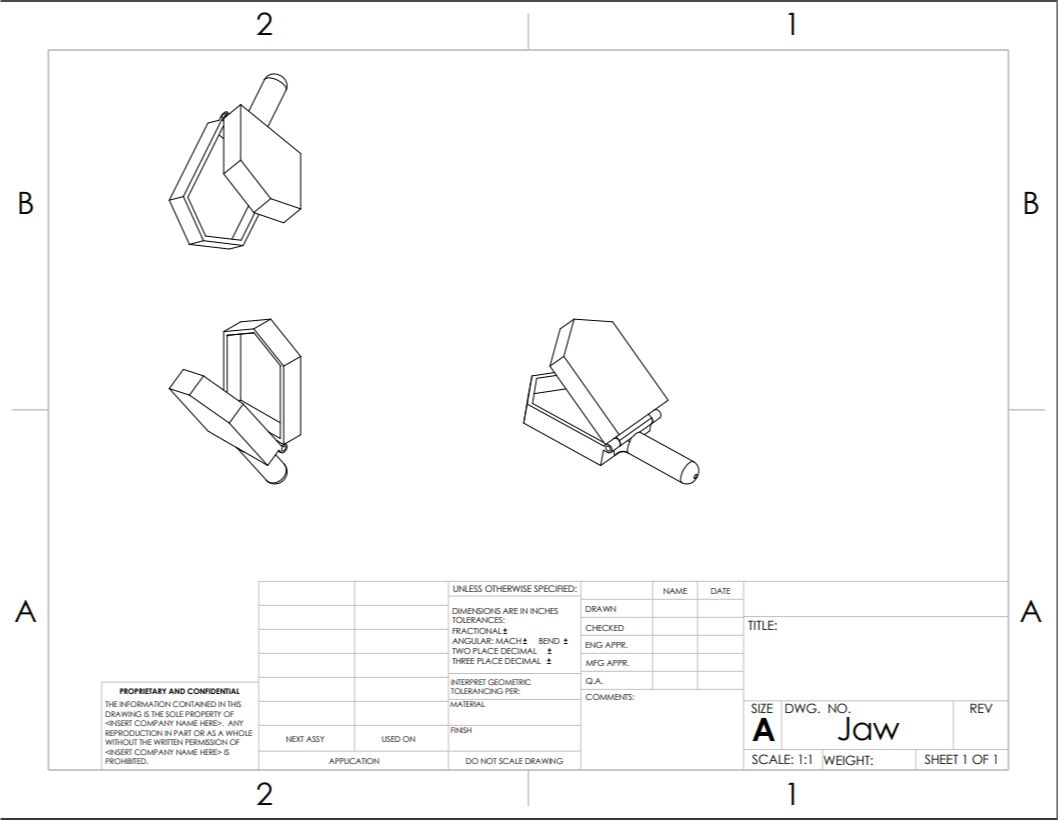
\includegraphics[width=0.8\columnwidth]{figures/fig733.png}
\end{center}
\caption{A digital drawing of the new Pac-Man design}
\label{fig:7.3.3}
\end{figure}

\begin{figure}
\begin{center}
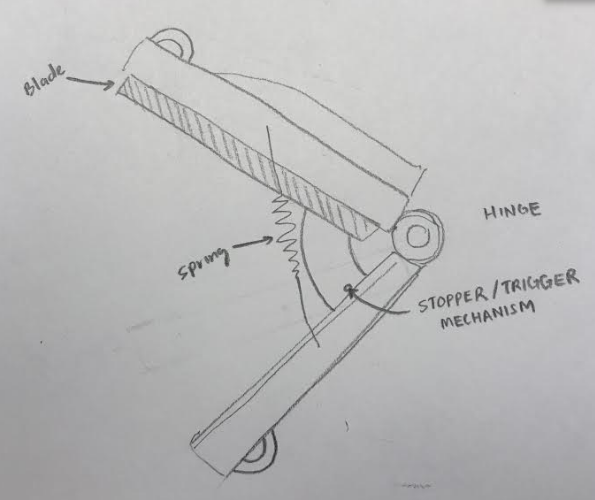
\includegraphics[width=0.8\columnwidth]{figures/fig734.png}
\end{center}
\caption{Prototype sketch of revised pac man design with parts labelled}
\label{fig:7.3.4}
\end{figure}

The location for the cutter system had to be outside of the rotor wash generated by the rotors that were closest to it.  Therefore, it was decided that the bar would extend about \SI{500}{\milli\meter} from the drone center (\fref{fig:7.3.5}). 
\begin{figure}
\begin{center}
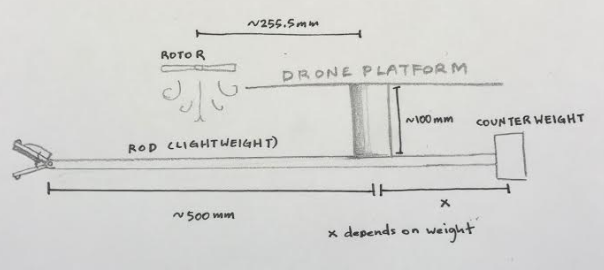
\includegraphics[width=\columnwidth]{figures/fig735.png}
\end{center}
\caption{Prototype drawing of complete pac man design}
\label{fig:7.3.5}
\end{figure}
 
After discussing the Pac-Man design with the workers at the Machine Shop, it was decided that the 
\begin{figure}
\begin{center}
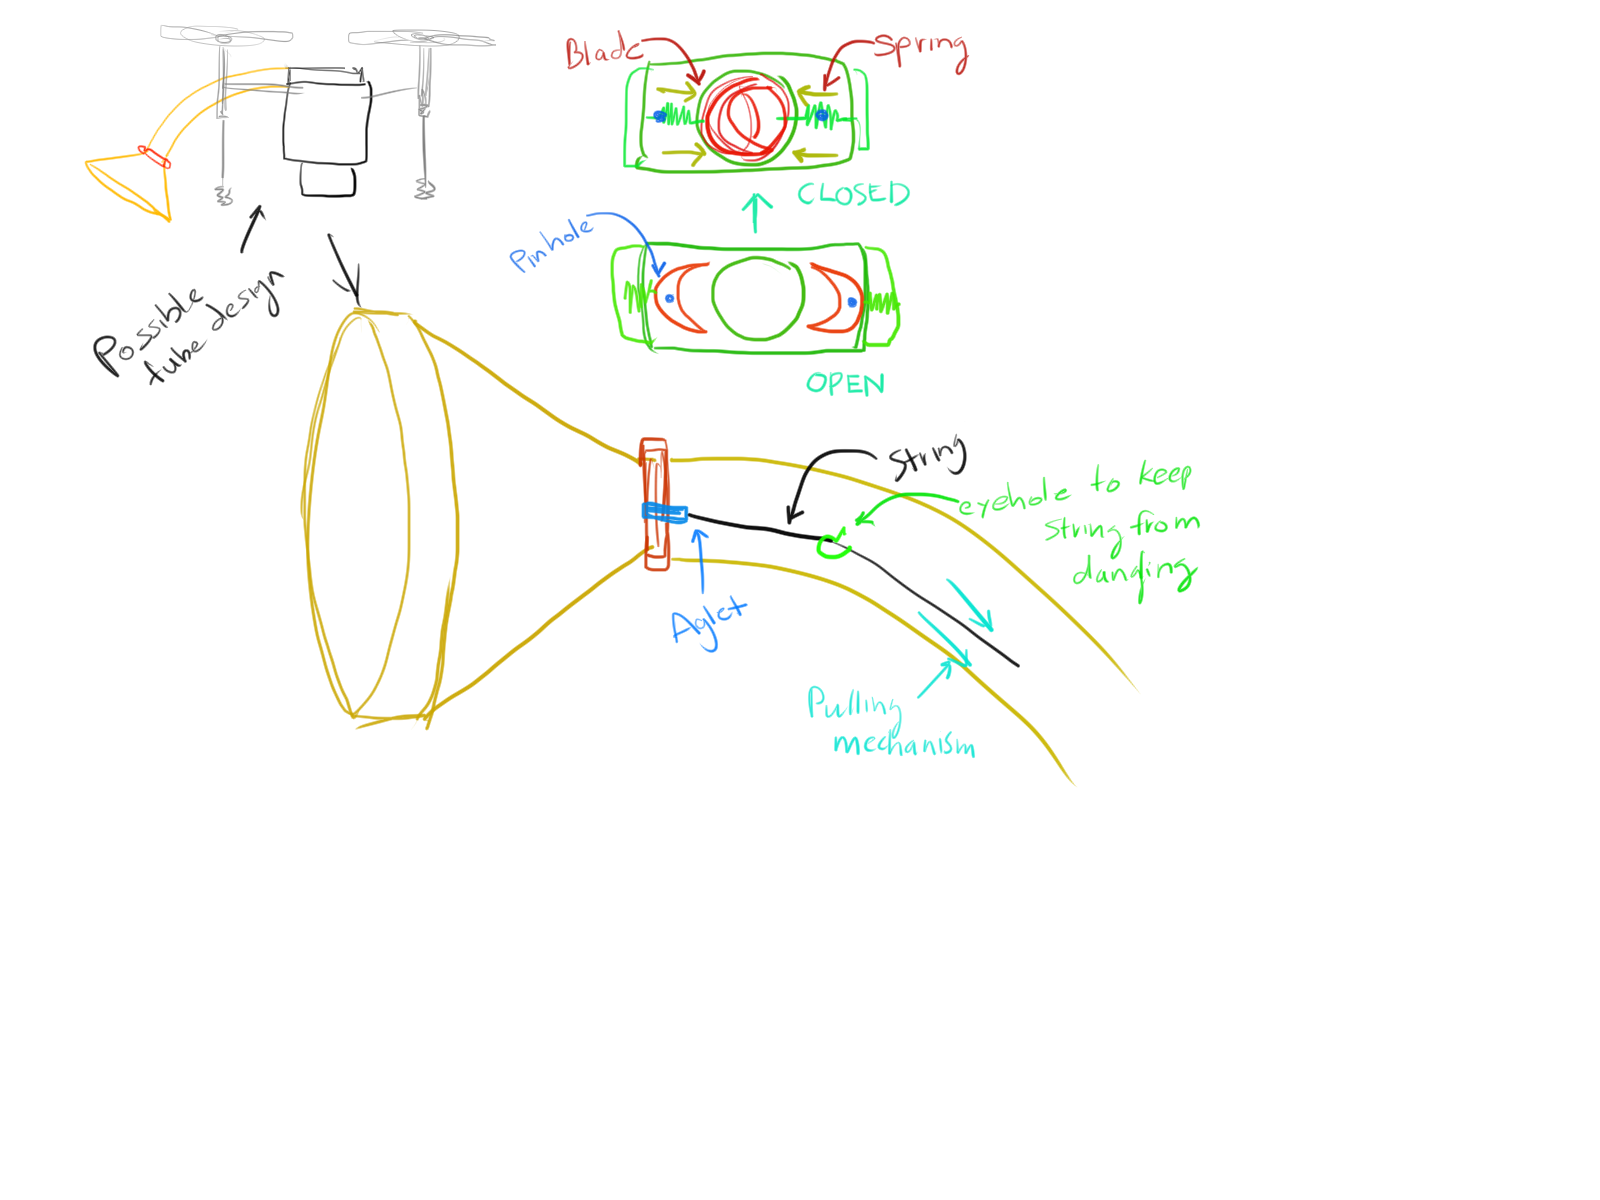
\includegraphics[width=\columnwidth]{figures/fig736.png}
\end{center}
\caption{Initial prototype drawing of cigar cutter extraction mechanism with tube and cone}
\label{fig:7.3.6}
\end{figure}
\begin{figure}
\begin{center}
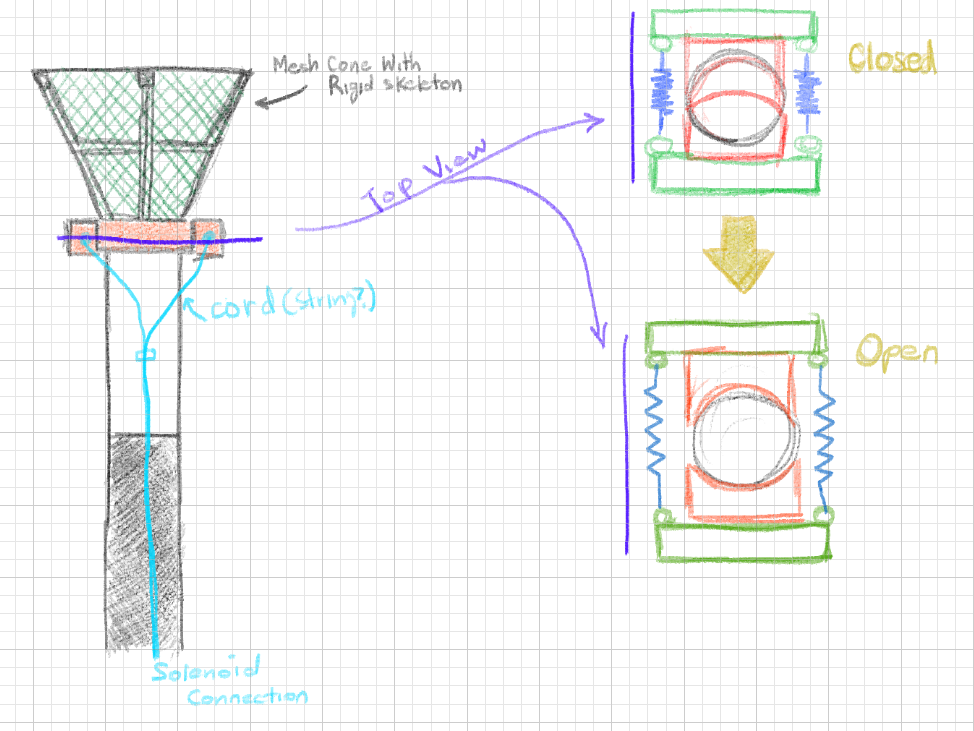
\includegraphics[width=\columnwidth]{figures/fig737.png}
\end{center}
\caption{Additional prototype sketch with solenoid concept included in cigar cutter}
\label{fig:7.3.7}
\end{figure}
\begin{figure}
\begin{center}
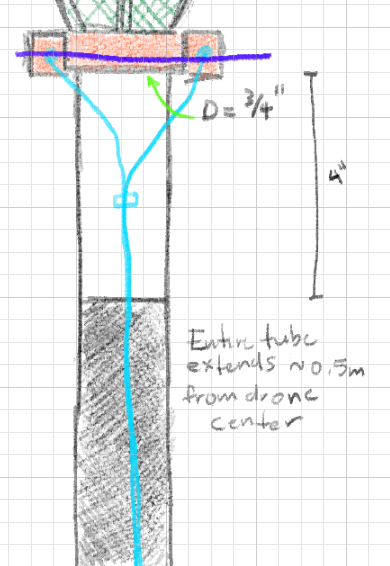
\includegraphics[width=0.49\columnwidth]{figures/fig738a.png}
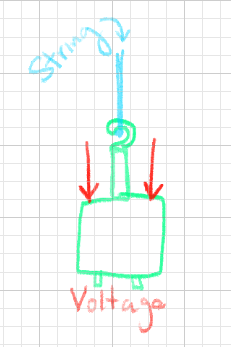
\includegraphics[width=0.49\columnwidth]{figures/fig738b.png}
\end{center}
\caption{More sketches of cigar cutter prototype with external power source for activation}
\label{fig:7.3.8}
\end{figure}
\begin{figure}
\begin{center}
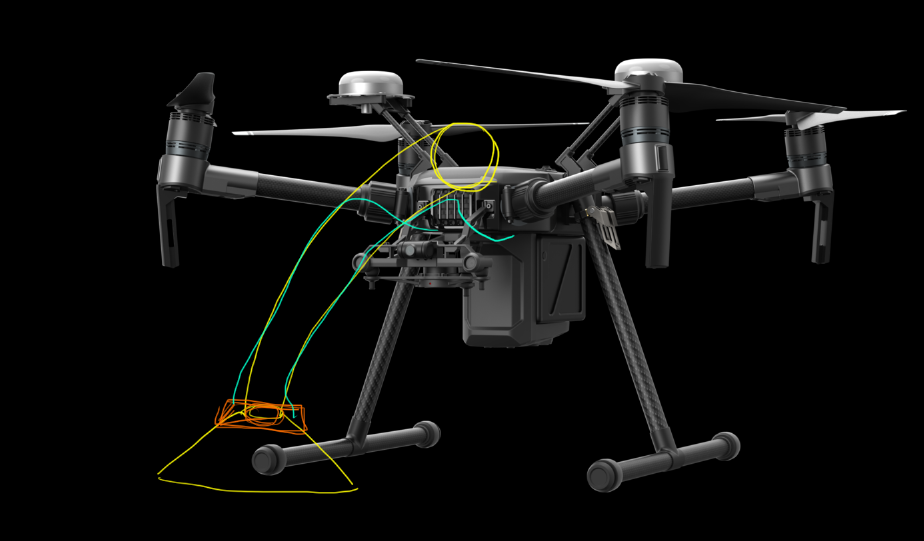
\includegraphics[width=\columnwidth]{figures/fig739.png}
\end{center}
\caption{Prototype sketch of final product prototyping}
\label{fig:7.3.9}
\end{figure}
\begin{figure}
\begin{center}
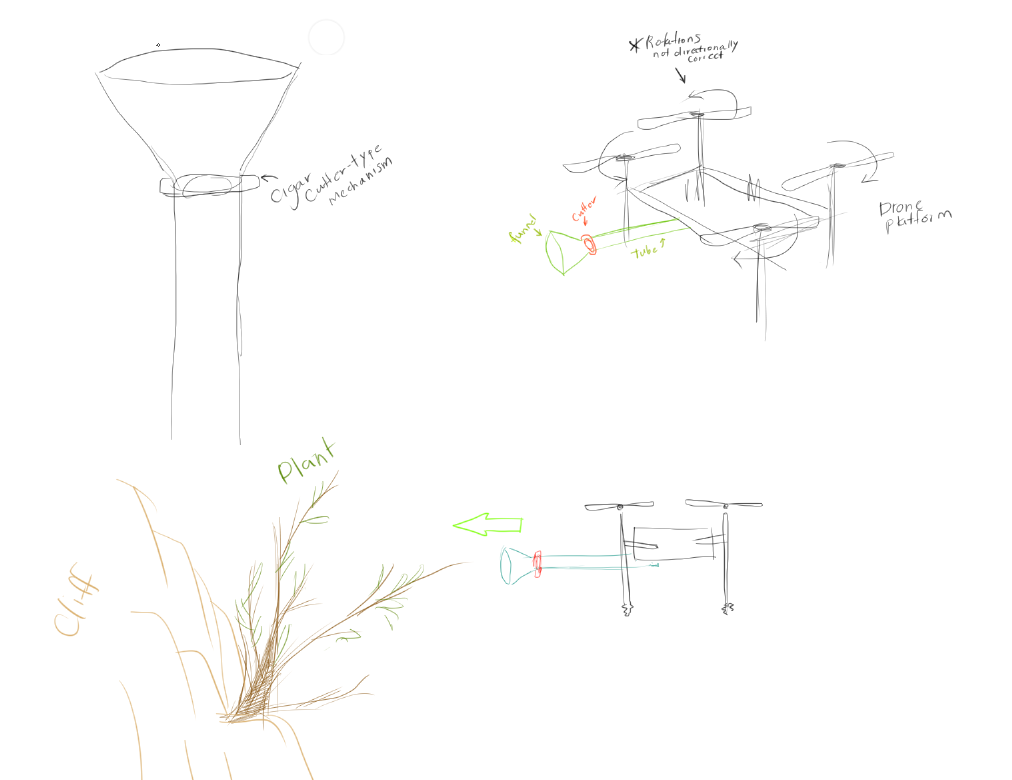
\includegraphics[width=0.8\columnwidth]{figures/fig7310.png}
\end{center}
\caption{Additional sketch of final product prototyping}
\label{fig:7.3.10}
\end{figure}
\begin{figure}
\begin{center}
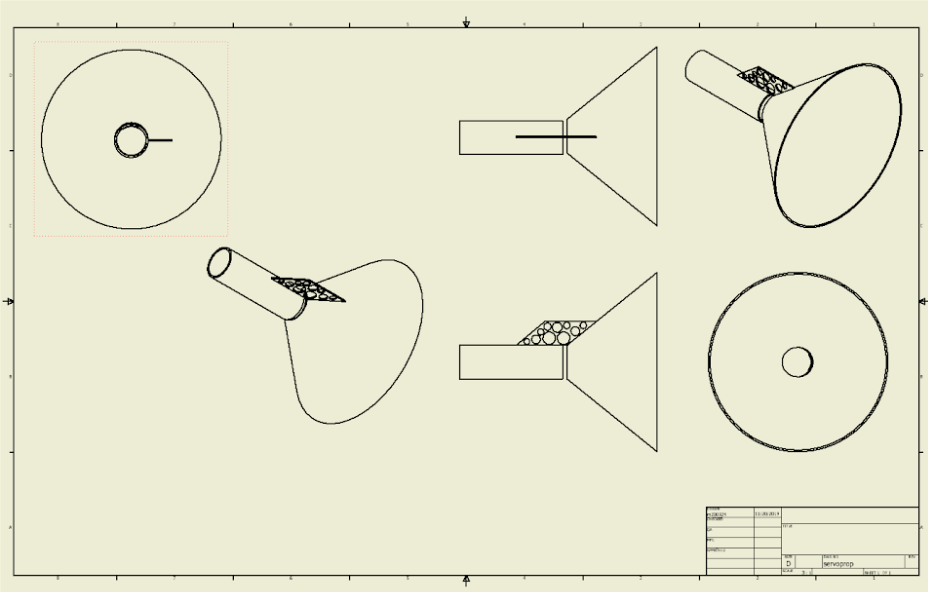
\includegraphics[width=\columnwidth]{figures/fig7311.png}
\end{center}
\caption{Digital prototype design for cone and tube if there were to be a servo attached.}
\label{fig:7.3.11}
\end{figure}





\subsection{Circuit Diagrams}
\begin{figure}
\begin{center}
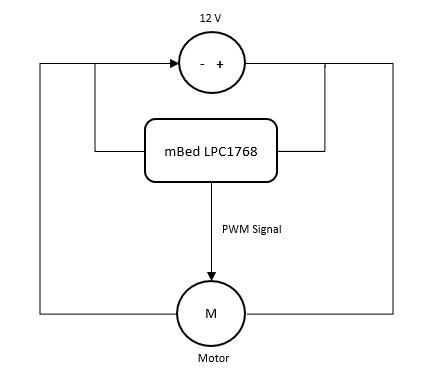
\includegraphics[width=0.6\columnwidth]{figures/fig741.png}
\end{center}
\caption{Basic Circuit Diagram of the Extraction Device}
\label{fig:7.4.1}
\end{figure}

\Fref{fig:7.4.1} shows the circuitry for the extraction device with a \SI{12}{\volt} power source, an LPC1768 microcontroller, and a motor. The LPC1768 has a recommended voltage input of \SIrange{4.5}{9}{\volt}, but it can function, with increased heat conversion, as long as the current is kept under \SI{150}{\milli\ampere}. as  We will use a \SI{12}{\volt} Motor to spin our end effector which is in parallel to the LPC 1768. The LPC 1768 will send a fixed PWM signal to the motor when prompted by the user.

This circuit represents the extraction device at a prototype level. In the air, the user will have to prompt the LPC1768 through wireless or radio communication. In the future, we will test with RC transmitters and receivers and incorporate them in the circuit to simulate a UAS in the air. 
\begin{figure}
\begin{center}
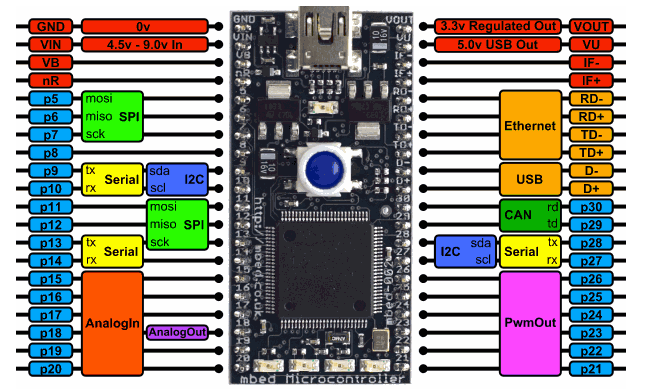
\includegraphics[width=\columnwidth]{figures/fig742.png}
\end{center}
\caption{Pin Allocations for the mbed LPC1768 Microcontroller \cite{mbed2019}}
\label{fig:7.4.2}
\end{figure}





\subsection{Prototypes}

\subsubsection{Parrot Bebop UAS}
\begin{figure}
\begin{center}
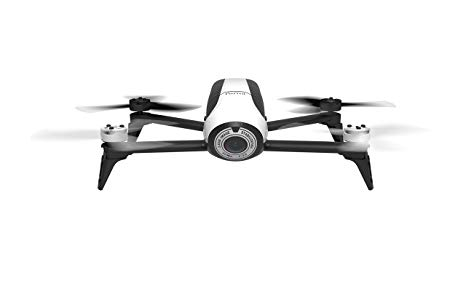
\includegraphics[width=0.3\columnwidth]{figures/fig751.png}
\end{center}
\caption{Parrot Bebop UAS \cite{parrot2019parrot}}
\label{fig:7.5.1}
\end{figure}
The Parrot Bebop UAS is a small scale prototype of the DJI Matrice 100. Testing on the prototype included video recording and putting a mock extraction device and see how it flew. This was before the DJI Matrice 100 was available for use. 

\subsubsection{Cigar Cutter Prototype}
\begin{figure}
\begin{center}
\includegraphics[height=1.3in]{figures/fig752a.png}
\includegraphics[height=1.3in]{figures/fig752b.png}
\includegraphics[height=1.3in]{figures/fig752c.png}
\end{center}
\caption{Cigar Cutter Prototype}
\label{fig:7.5.2}
\end{figure}
The cigar cutter prototype is fully functional and is able to accurately and reliably cut through stems. The plants are fed through the cigar cutter through a cone and are then cut using power from a set of springs.  Despite being a fully functional the design will need to be improved before it is ready to be mounted to the quadcopter.   

\subsubsection{Mouse Trap Prototype}
\begin{figure}
\begin{center}
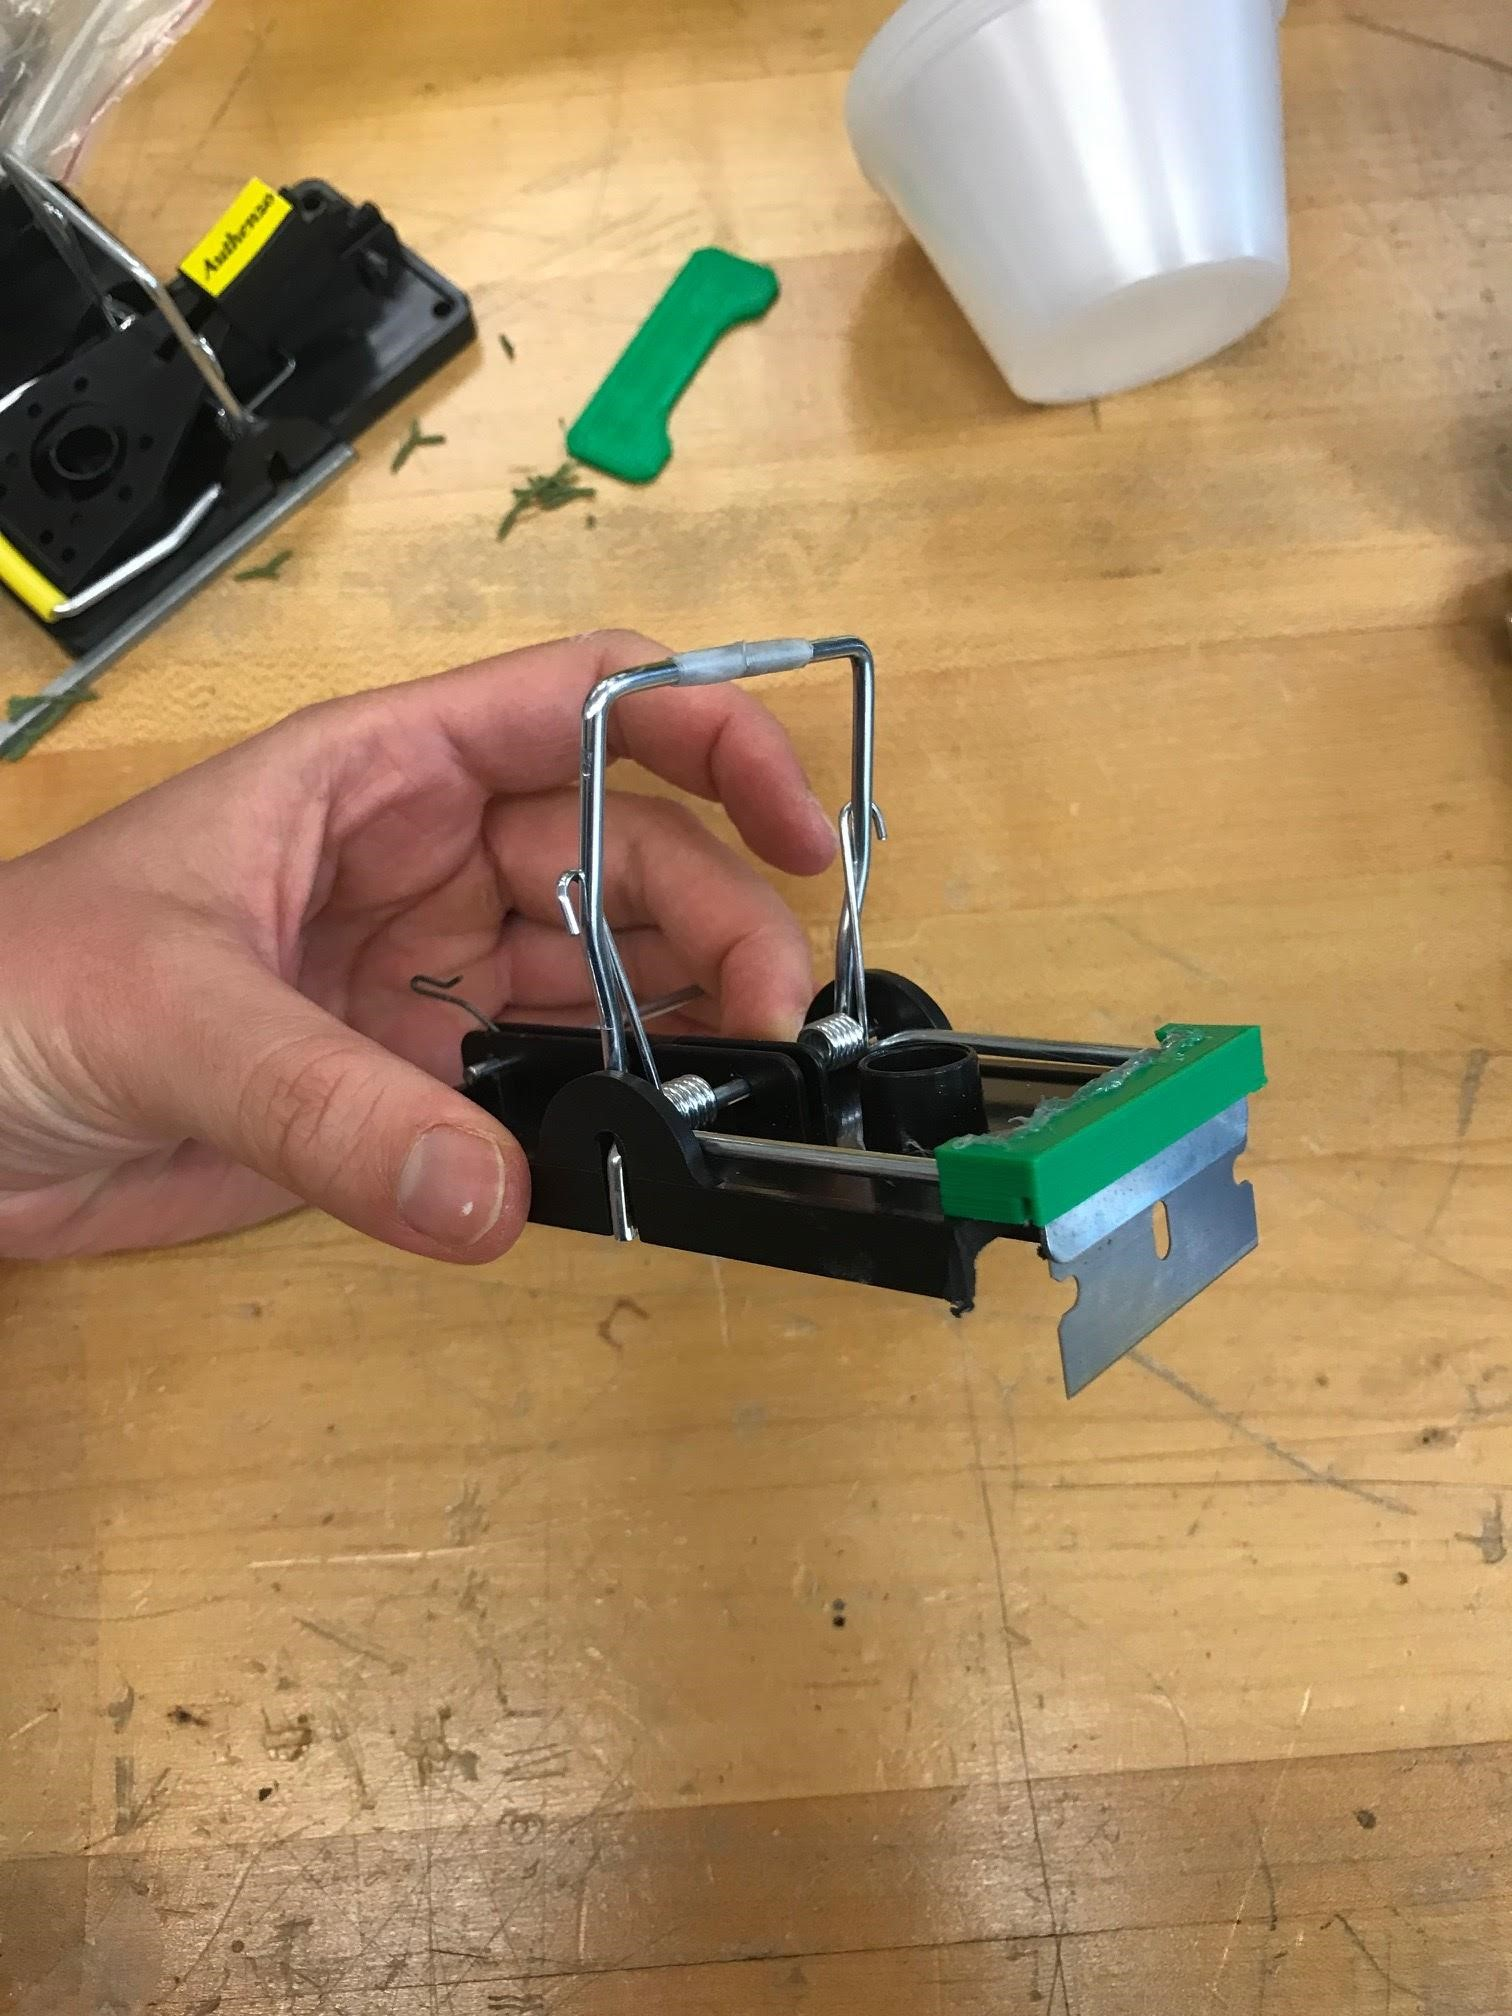
\includegraphics[width=0.5\columnwidth]{figures/fig753.jpg}
\end{center}
\caption{Mouse Trap Prototype}
\label{fig:7.5.3}
\end{figure}
The Mouse Trap Prototype is designed to cut through the plant with shear force as there is a blade attached to the mouse trap to ensure the plant is cut successfully. The mouse trap is positioned to the plant and when activated via a signal, the mouse trap prototype will close in on the plant snapping the sample from the main stem. 

\subsubsection{Mythbusters Motor Driven Shear and Servo Driven Gripper}
As seen in \fref{fig:7.5.4}, %??figure 4.5.1
the Motor Driven Sheer and Servo Driven Gripper are designed to more accurately cut and grip our desired plant. The motor drives a shaft connected to a worm drive. The worm drive will turn a gear that creates a linear motion through links that will moves the shears to open and close. Furthermore we will have a servo driven gripper placed on top of the shear to simultaneously grab onto the plant.
\begin{figure}
\begin{center}
\includegraphics[width=0.4\columnwidth]{figures/fig754a.png}
\includegraphics[width=0.4\columnwidth]{figures/fig754b.png}
\end{center}
\caption{Motorized Shear Prototype}
\label{fig:7.5.4}
\end{figure}





\subsection{Software Structure}
\begin{figure}
%\begin{center}
%\includegraphics[width=0.8\columnwidth]{figures/fig761.png}
%\end{center}
\lstinputlisting[style=mbedC]{code/mbed/motor-control/main.cpp}
\caption{Pseudocode for the mbed LPC1768 Microcontroller to Control a Motor}
\label{fig:7.6.1}
\end{figure}

The pseudocode in \fref{fig:7.6.1} shows the process of controlling a motor at the prompt of the user. The mbed continually sends PWM signals through a conditional while loop. When prompted by the user to start the motor, the mbed will send a higher PWM signal to the motor and change the variable which controls the while loop conditional. Another prompt will change the variable back to 0 which brings the code back to the original while loop.




\subsection{Simulations}

The simulations we conducted are more related towards how the operation would go if the group was in California. We simulated the test environment on Hospital Point with what was available to emulate the beginning of the UAS operation to the end. We measured out and taped the dimensions of the powered boat we would be on (\SI{20 x 6}{\foot}) and a ``landing platform'' on the side of the boat (\SI{6 x 6}{\foot}) where the UAS would take off and land from. 

In a Line of Sight Maneuver and live-stream received from the gimbal on the UAS, the UAS pilots (1/C Jisub Lim and 1/C Bryan) flew the UAS from the landing platform and tested out how the resolution was from the gimbal by flying close to the trees on Hospital Point. Afterwards, the UAS pilot conducted a landing maneuver onto the landing platform and timing how long it took to successfully land the UAS.

Other simulations/tests included battery life during flight maneuvers, testing the range of how far the UAS could go from the boat, and max speed tests as well. 

In regards to simulations for the extraction device, there are currently two prototypes that have been simulated. The mouse trap and cigar cutter extraction devices were manually held by hand. With a sample plant to test the extraction devices, the device was triggered by hand. We observed and recorded how the plant was cut. These are the simulations that have been conducted to emulate the subcomponents of the UAS and UAS operation. 







\section{Proposed Work}

\subsection{Work Breakdown Structure}
\begin{table}
\caption{Work Breakdown for each Team member}
\label{tab:8.1.1}
\begin{center}
\includegraphics[width=\columnwidth]{figures/table-811.jpg}
\end{center}
\end{table}

\subsection{Timeline}
\begin{table}
\caption{Timeline}
\label{tab:8.2.2}
\begin{center}
\includegraphics[width=0.8\columnwidth]{figures/table-821.png}
\end{center}
\end{table}

\clearpage
\begin{figure}
\begin{center}
%\includegraphics[angle=90,width=\columnwidth]{figures/table-822.png}
\includegraphics[width=\columnwidth]{figures/gantt.png}
\end{center}
\caption{Gantt Chart}
\label{tab:8.2.3}
\end{figure}





\subsection{Risk management}
\begin{table}
\caption{Risk of dropping UAS in water}
\label{tab:8.3.1a}
\includegraphics[width=\columnwidth]{figures/table-831a.jpg}
\end{table}

\begin{table}
\caption{Risk of not cutting plant completely}
\label{tab:8.3.1b}
\includegraphics[width=\columnwidth]{figures/table-831b.jpg}
\end{table}

\begin{table}
\caption{Risk of running out of battery / flight time}
\label{tab:8.3.1c}
\includegraphics[width=\columnwidth]{figures/table-831c.jpg}
\end{table}

\begin{table}
\caption{Risk of collision}
\label{tab:8.3.1d}
\includegraphics[width=\columnwidth]{figures/table-831d.jpg}
\end{table}

\begin{table}
\caption{Risk of crew overboard}
\label{tab:8.3.1e}
\includegraphics[width=\columnwidth]{figures/table-831e.jpg}
\end{table}

\begin{table}
\caption{Risk of actuation failure of snipper}
\label{tab:8.3.1f}
\includegraphics[width=\columnwidth]{figures/table-831f.jpg}
\end{table}

\begin{table}
\caption{Risk of getting lost at sea}
\label{tab:8.3.1g}
\includegraphics[width=\columnwidth]{figures/table-831g.jpg}
\end{table}

\begin{table}
\caption{Risk of injury while recovering UAS}
\label{tab:8.3.1i}
\includegraphics[width=\columnwidth]{figures/table-831i.jpg}
\end{table}









\subsection{Demonstration and Testing Plan}
For the UAS subsystem, we have tested what is possible to test for the UAS as of right now. We have recordings of the UAS taking and landing off through the tablet interface as well as one of us recording from the ground. The UAS battery life/operating time, max height and range, and the live-stream interface from the UAS have been observed and recorded during the test. We are devising a safe method to test the max payload capacity the UAS can hold since we are not able to attach the extraction device onto the UAS yet. With the recorded values of the tests conducted, they will be observed compared to the metrics and score it based on where it falls into the metrics.

For the extraction device, we will demonstrate the prototypes that we have made so far: the mousetrap, cigar cutter, and motorized shear extraction device prototypes. We will repeat the testing that’s been done on the three extraction devices with a sample plant to determine which one we will invest our resources into. The extraction device is configured into a circuit powered by an external battery/power source and controlled by an mbed microcontroller. Based on the metric parameters, such as the number of trials, the extraction device can be tested and we can observe the success rate of the different prototypes.








\section{Benchtop Demonstration}
\subsection{Activities}
During the final weeks of the semester, the extraction device team, Reina, Bryan and Levi, continued researching and designing for the extraction device prototypes, the three main designs being the mouse trap, motor driven snipper, servo driven gripper and cigar cutter devices. Jacob has a working circuit board that is available to test motors or servos connected to an extraction device to electrically power the extraction device. Jisub and Bryan are working on the UAS, getting flight time, and looking into other prototypes for the extraction device. We have also tested the live-stream from the UAS’s gimbal camera and marking certain distances and seeing how far the UAS can be while being able to identify a certain target which would be the plant. 
        
\subsection{Results}
\subsubsection{Operation simulation}
Test: Operation Simulation
Date: \printdate{11/21/2019}
Air Temperature: \SI{41}{\fahrenheit}
Experiment: The layout of the \SI{20x6}{\foot} power driven vessel was outlined in the grass of the field using masking tape. The boat that we will be training with has a maximum passenger capacity of 10. Our planned this test with seven passengers and the stern of the boat used for equipment. The passenger zone and the takeoff/landing zone was separated.  Available team members were positioned in the passenger section based on their role in UAS operations to test space availability during operations. Jacob is the boatswain, Ji is the pilot, Bryan is the Co-Pilot, Reina and Levi are note takers and safety observers. We made room for two other passengers on the boat. The goal of this test was to test safety during operations on a boat, space availability on the boat, and a full concept simulation of our operations.

Takeaways: 

During the operation simulation, we found that the DJI Matrice 100 UAS is very stable during flight and there were no issues with connection to the UAS at any range. Surveying the trees and surrounding environment showed positive results in which the quality of the camera was pretty good. We tested how close we could get to the trees and saw that the down drift on the UAS doesn’t affect the trees unless the UAS is directly above the tree. 

Landing maneuvers were conducted for both pilots (1/C Jisub and 1/C Bryan) and both landings were successful. We measured the distance from the center of the landing platform to the center of the drone. The data for that is discussed further below in the report. The space availability on the mock up of the boat was adequate, but there is a need for consideration of what type of boat we will be using in California as compared to the powered boat that is available at USNA. 
\begin{figure}
\begin{center}
\includegraphics[width=0.5\columnwidth]{figures/fig921.png}
\end{center}
\caption{A photo of the landing platform layout}
\label{fig:9.2.1}
\end{figure}
\begin{figure}
\begin{center}
\includegraphics[width=0.5\columnwidth]{figures/fig922.png}
\end{center}
\caption{A photo of the STEVE team simulating UAS operations from the boat}
\label{fig:9.2.2}
\end{figure}




\subsubsection{Battery life test}
Test: Battery Life
\begin{figure}
\begin{center}
\includegraphics[width=\columnwidth]{figures/fig923.png}
\end{center}
\caption{A graph showing the battery life of the TB48D (blue) and the TB47D (orange)}
\label{fig:9.2.3}
\end{figure}

The UAS was flown arbitrarily in increments of a few minutes in order to determine the actual battery life of the current UAS battery.  Each flight was a mixture of hovering and moving in order to familiarize the pilot (Jisub Lim) with the operation of the UAS.  The time and battery life after each flight was recorded.  The chart below shows the battery life against time for each test.  The blue line is the data for the flights done at small increments (\SIrange{2}{5}{\minute}) at a time using the TB48D battery, and the orange line shows the data for a longer flight made to deplete the battery completely (TB47D battery).

Takeaways:  

The battery life was shorter than the advertised battery due to varying conditions and likely due to wear. The battery may have been affected by the cold temperatures of the air. The UAS automatically lands when it hits 10\% battery life. The gimbal was not centered on the UAS platform, so there was always a slight offset when landing using only the camera




\subsubsection{Strength of twings}
Test: Strength of Twigs

Experiment: Using the purchased cigar cutter, twigs of different thicknesses will be tested in order to determine the relationship between the twig diameter and the force required to cut the twig.

In order to test how much force it takes to cut the branch, a scale was placed underneath the cigar cutter.  The blades were opened, the branch was fed into the hole, and the blades were pushed together by the scale on the bottom, and the hand on top.  The cedar branch was used because it is a fibrous plant that is harder to cut than most other plants.  Knowing the force required to cut each diameter can help us determine the amount of force our design needs to apply.  The test was conducted on two different plants: the cedar and the unknown softer twig.
\begin{table}
%\begin{center}
%\includegraphics[width=\columnwidth]{figures/table-921.png}
%\end{center}
\caption{Table testing required force to cut various twigs of various diameters}
\label{tab:9.2.1}
\begin{center}
\begin{tabular}{ccc}
\toprule
& twig diameter, \si{\milli\meter} & force to cut, \si{\poundforce} \\
\midrule
cedar & 4.9 & 34, 35, 38$_1$\\
cedar & 3.85 & 18 \\
cedar & 3.8 & 16 \\
cedar & 3.61 & 17 \\
cedar & 3.58 & 15 \\
cedar & 3.39 & 14 \\
cedar & 3.10 & 13 \\
softer & 1.66 & 0.31 \\
softer & 2.12 & 0.69 \\
softer & 2.4 & 0.81 \\
softer & 2.82 & 4 \\
softer & 3.06 & 9 \\
softer & 3.53 & 11, 11, 12$_1$\\
softer & 3.79 & 14 \\
softer & 3.75 & 14 \\
softer & 4.48 & 24 \\
softer & 4.56 & 24 \\
softer & 4.76 & 26 \\
\bottomrule
\end{tabular}
\vspace{2em}

$^1$multiple tests of same diameter
\end{center}
\end{table}


\begin{figure}
\begin{center}
\includegraphics[width=\columnwidth]{figures/fig924.png}
\end{center}
\caption{A graph showing the force required to cut vs the diameter of the branch}
\label{fig:9.2.4}
\end{figure}

Takeaways:
Branches are pretty hard to cut with a cigar cutter (sometimes the force required was close to \SI{40}{\poundforce}). There is some space between the blades that may cause slim, long, and flexible plants to deflect and not be cut fully. Clearly, the force increased with diameter, but the relationship was not linear

Imperfections of the experiment: The experiment only tests the twigs available to us in Annapolis.  The twigs that we will be taking samples from will probably have a slightly different composition because they are of a different species.  This test hopefully will give us a good idea on how strong the spring system must be in order to cut almost any potential sample.



\subsubsection{Time and difficulty of landing}
  
Test: Time and Difficulty of Landing

Experiment:
Two UAS pilots practiced landing the UAS in the allotted \SI{6x6}{\foot} box. The time it took to land the UAS after flying was recorded for each flight. The landing maneuver was defined as when the pilot concentrates solely on getting back on the platform after flying the UAS back to the boat.
After landing, the distance of the center of the UAS from the center of the platform was recorded in order to determine the offset caused by the location of the gimbal.  This bench test was also used in order to determine the best/most accurate UAS pilot for the experiment.

\begin{table}
\caption{Landing time and distance from platform center measurement for each UAS pilot}
\label{tab:9.2.2}
\begin{center}
\begin{tabular}{lll}
\toprule
landing time, \si{\second} & distance from platform center & UAS pilot \\
\midrule
48 & 8 & Ji \\
70 & 8 & Ji \\
90 & 12 & Bryan \\
95 & 15 & Bryan \\
\bottomrule
\end{tabular}
\end{center}
\end{table}
 
Takeaways: 
Jisub performed better as the UAS pilot than Bryan. The UAS lands automatically with the return-to-home feature which will not be applicable when the boat is moving. Angling the camera at \ang{90} is an accurate way to land manually. The other team members on the boat can assist with the landing of the drone as well. The UAS lands automatically at 10\% battery regardless of location, but there are a series of alarms and notifications before this happens.





\nocite{hyneman2017jamie, famoussmoke2019cigar} % never used? 
%\section{References}
\bibliography{biosteve.bib}





% Appendices here (optional)
%\clearpage
%\appendix
%\renewcommand{\figurename}{Supplementary Figure}
%\renewcommand{\thefigure}{S\arabic{figure}}
\end{document}